\documentclass{article}

\usepackage{microtype}
\usepackage{graphicx}
\usepackage{subcaption}
\usepackage{booktabs}
\PassOptionsToPackage{hyphens}{url}
\usepackage{hyperref}
\newcommand{\theHalgorithm}{\arabic{algorithm}}

% For blind submission:
\usepackage{icml2026}
% For camera-ready: \usepackage[accepted]{icml2026}

\usepackage{amsmath}
\usepackage{amsfonts}
\usepackage{amssymb}
\usepackage{xcolor}
\usepackage{float}
\usepackage{tabularx}
\usepackage{multirow}
\usepackage{url}

\definecolor{darkblue}{rgb}{0, 0, 0.5}
\hypersetup{colorlinks=true, citecolor=darkblue, linkcolor=darkblue, urlcolor=darkblue}

\newcommand{\fix}{\marginpar{FIX}}
\newcommand{\new}{\marginpar{NEW}}

\icmltitlerunning{Where's the Plan? Locating Latent Planning in Language Models with Lightweight Mechanistic Interventions}

\setlength{\emergencystretch}{3em}

\begin{document}

\twocolumn[
  \icmltitle{Where's the Plan? Locating Latent Planning in Language Models with Lightweight Mechanistic Interventions}

  \begin{icmlauthorlist}
    \icmlauthor{Author 1}{stanford}
    \icmlauthor{Author 2}{stanford}
  \end{icmlauthorlist}

  \icmlaffiliation{stanford}{Stanford University, Stanford, CA, USA}

  \icmlcorrespondingauthor{Author 1}{author@example.com}

  \icmlkeywords{mechanistic interpretability, latent planning, language models, activation patching, probing}

  \vskip 0.3in
]

\printAffiliationsAndNotice{}

\begin{abstract}
Prior work establishes that language models exhibit latent planning---but \textit{where and how} do planning mechanisms form in the network? We introduce the notion of \textit{planning site formation} and investigate it across Qwen3, Gemma-3, and Llama-3 model families at more than ten scales using linear probing and activation patching on rhyming couplet generation. Probing reveals that planning-compatible representations emerge at the newline token with scale across all three families, yet their strength and layer profile vary substantially across architectures. Activation patching reveals a sharp dissociation: only Gemma-3-27B forms a causally active planning site at the newline, via a representational handoff in which causal influence migrates from the last word token to the newline mid-network. We further localize this handoff to a sparse set of five attention heads that jointly account for ${\sim}73\%$ of the full patching effect. All other models, including all Qwen3 sizes up to 32B and all Llama-3 sizes up to 8B, condition on the last word token throughout generation despite exhibiting strong probe signal, showing that planning-compatible representations do not imply causal planning behavior. Our activation patching approach requires no transcoder training and far less data than steering vector approaches, making it a scalable framework for studying latent planning across architectures.
\end{abstract}


\section{Introduction}

Autoregressive language models generate text one token at a time, yet routinely produce outputs requiring long-range structural coherence. Rhyming couplets, for example, require that tokens generated late in the sequence stand in a precise phonological relation to a stimulus word from much earlier. This raises a natural question: do models form internal representations of future outputs that causally shape generation, entirely invisible to behavioral evaluation? We call this \textit{latent planning}. Unlike chain-of-thought reasoning~\citep{wei2022chain}, where intermediate steps are directly observable, latent planning occurs entirely within a model's hidden activations. If models are planning in ways invisible to external observers, standard behavioral evaluations may systematically underestimate this capacity, making it both a scientific and a safety-relevant problem~\citep{pfau2024dots,hao2024coconut}.

Neural networks trained on next-step prediction can develop internal planning representations in structured domains. McGrath et al.~\citeyearpar{mcgrath22} find that chess concepts emerge in AlphaZero's internal layers; Li et al.~\citeyearpar{li24} and Nanda et al.~\citeyearpar{nanda23} show that transformers trained on Othello develop linear, causally manipulable board representations; and Jenner et al.~\citeyearpar{jenner24} provide mechanistic evidence of learned look-ahead in a chess-playing network. These results motivate the question of whether language models elicit analogous mechanisms during open-ended generation. Prior work on large language models establishes that planning-compatible information exists in some models~\citep{maar2026whatsplanmetricsimplicit,hanna2026latent,dong2025emergentresponseplanningllms,pochinkov2025parascopeslanguagemodelsactivations}, but does not address a more specific question: \textit{where exactly does planning information reside during the forward pass, and does it move?} We call this \textbf{planning site formation}.

Investigating planning sites rigorously requires both encoding evidence (what information is present) and causal evidence (what information is used). Probes assess what is encoded in hidden states~\citep{hewitt19,burns24}, but sufficiently flexible probes can achieve high accuracy by memorizing labels rather than reflecting genuine representations~\citep{hewitt19}. Causal tools such as activation patching~\citep{meng23,wang2022ioi} and steering vectors~\citep{turner2023activation,arditi2024refusal} are needed to establish that encoded information actually influences downstream generation. The most expressive existing approach, training transcoders~\citep{transcoders} to build feature circuits~\citep{sparsefeaturecircuits,ameisen2025circuittracing}, provides fine-grained circuit analysis but requires substantial compute (effectively a second training run), has so far been applied only to closed-source models such as Claude 3.5 Haiku~\citep{anthropic-bio}, and does not straightforwardly scale to new open-source architectures. Work by \citet{maar2026whatsplanmetricsimplicit} uses steering vector interventions and finds most open-source models up to 30B parameters keep their planning sites at the last word token; a transcoder-based analysis by \citet{anthropic-bio} on Claude 3.5 Haiku finds evidence of a planning site migrating to the newline. These results motivate a scalable framework for studying planning site formation across model architectures and scales.

In this paper, we define two notions for surfacing evidence of latent planning: the weaker notion of planning-compatible representations (detectable via probing) and the stricter notion of causally active planning sites (established via activation patching). Using only linear probing and activation patching (requiring no transcoder training and far less data than steering vector approaches), we investigate planning site formation across three open-source model families at multiple scales (up to 32B parameters).

Probing reveals that planning-compatible representations emerge at the newline token with scale across all three families, yet their strength and layer profile vary substantially across architectures. Activation patching reveals a sharp dissociation: only Gemma-3-27B forms a causally active planning site at the newline, exhibiting an information routing handoff in which causal influence migrates from the last word token to the newline around layer 30. All other models, including all Qwen3 sizes up to 32B and all Llama-3 sizes up to 8B, condition on the last word token throughout generation despite encoding planning-compatible representations at the newline. We further localize the handoff in Gemma-3-27B to a sparse set of five attention heads spanning layers 28--34, identified via attention weight ranking and simultaneous head patching. This suggests that planning site formation is a distinct emergent phenomenon tied to specific model scale and architecture, rather than a general consequence of strong planning-compatible representations.


\section{Setup and Notation}
\label{sec:2}
In this paper, we study rhyming couplet generation as an example of latent planning.
A rhyming couplet is a two-line poem where the last word of the first line, denoted $r_1$, rhymes with the last word of the second line, denoted $r_2$.
We task language models to complete rhyming couplets, (i.e., given context containing $r_1$, generate a completion where $r_2$ rhymes with $r_1$). For example, given the prompt \texttt{"A rhyming couplet:\textbackslash nShe felt a sudden sense of fright,\textbackslash n"}, the model should produce a completion such as \texttt{"and hoped that dawn would end the night.\textbackslash n"}, where $r_1 = \texttt{fright}$ and $r_2 = \texttt{night}$.

Consider an autoregressive transformer language model with $L$ layers and hidden dimension $d$.
Let $\mathbf{h}_{\ell,i} \in \mathbb{R}^d$ denote the hidden state vector after the $\ell$-th transformer block at position $i$.
We adopt a relative positioning scheme centered around the newline token $\verb|\n|$ ending the first line of the couplet.
We refer to this token as being at position 0, with position $i$ referring to an offset of $i$ behind/ahead of the newline.

We say $(i, \ell)$ contains a \textit{planning-compatible representation} if the generated $r_2$ can be decoded from $\mathbf{h}_{\ell,i}$ via probing substantially better at position $i$ than at other positions.
This signals information about the future token and/or rhyme scheme is disproportionally encoded at the location $(i, \ell)$ compared to other hidden states.
As a stricter definition, we say $(i, \ell)$ is a \textit{causally active planning site} if replacing $\mathbf{h}_{\ell,i}$ during generation with the hidden state from a run targeting a different rhyme substantially redirects output toward that rhyme.
This shows that rhyme information located at $(i, \ell)$ is causally used in generation.


\section{Probing for Planning-Compatible Representations}
\label{sec:probing}
To investigate planning-compatible representations, we train linear probes to predict future tokens from hidden states.
Let $\mathcal V$ be the vocabulary (set of all tokens) and $\Delta \mathcal V$ the probability simplex over $\mathcal V$.
Each linear probe is a parameterized function $f_{(W,b)}(\mathbf{h}): \mathbb{R}^d \to \Delta \mathcal V$ where $f_{(W,b)}(\mathbf{h}) = \text{softmax}(W\mathbf{h} + \mathbf{b})$.
Probes are trained by minimizing cross-entropy loss. Probe parameters are optimized with AdamW~\citep{adamw} with learning rate $10^{-4}$, weight decay $10^{-3}$, batch size 32, for 10 epochs.

\subsection{Probing general text as a negative control}
\label{sec:probe-general}

We first verify that planning-compatible representations are task-specific and do not occur in general text generation.
We randomly sample 1,200 (1,000 train, 200 validation) token sequences from The Pile~\citep{thepile}, greedily sample model completions while storing activations to build the probe training dataset.
For each layer $\ell$ and various look-ahead distances $k$, we train a linear probe to predict the generated token at position $i+k$ from $\mathbf{h}_{\ell,i}$.
We compare against a baseline unigram model (trained on the corpus of all model completions) to ensure probes are learning more than just token frequencies.

\begin{figure*}[t]
    \centering
    \begin{subfigure}{0.325\linewidth}
        \centering
        \subcaption[]{Qwen3-32B}
        
\includegraphics[width=\linewidth]{media/results-probe/qwen-top5.png}
    \end{subfigure}
    \begin{subfigure}{0.325\linewidth}
        \centering
        \subcaption[]{Gemma-3-27B}
        
\includegraphics[width=\linewidth]{media/results-probe/gemma-top5.png}
    \end{subfigure}
    \begin{subfigure}{0.325\linewidth}
        \centering
        \subcaption[]{Llama-3.1-8B}
        
\includegraphics[width=\linewidth]{media/results-probe/gemma-top5.png}
    \end{subfigure}
    \caption{Top-5 accuracy of linear probes predicting $k$ tokens ahead in general text (Pile). Accuracy degrades monotonically with look-ahead distance $k$ and falls to the unigram baseline by $k=8$ across all layers, confirming that planning-compatible representations are not a generic feature of the residual stream.}
    \label{fig:probe-results}
\end{figure*}

We find probe accuracy degrades monotonically with $k$ and falls to baseline by $k=8$ across all
layers and both models (Figure~\ref{fig:probe-results}), confirming that
planning-compatible representations are not a generic property of the residual stream.
This provides a negative control establishing that probe signal in Section~\ref{sec:probe-couplets} is significant.

\subsection{Probing rhyming couplets}
\label{sec:probe-couplets}
For rhyming couplet generation, we first synthetically generate 1,200 (1,000 train, 200 validation) rhyming couplets with Claude Sonnet 4.6 \citep{sonnet46}, strategically prompting for diversity of topics and rhyme schemes.
We truncate the second line of each couplet, then greedily sample model completions for the second line, storing activations to build the probe training dataset.
We train probes to predict the rhyming token $r_2$ from $\mathbf{h}_{\ell,i}$ (Figure~\ref{fig:poem-diagram}), evaluating on raw accuracy and rhyme accuracy (as determined by the CMU Pronouncing Dictionary \citep{cmu}) across layers and positions.
The comparison is between probes trained on activations at the newline position ($i=0$) and subsequent positions ($i > 0$).
If a model constructs a planning-compatible representation at the newline before generation begins, the $i=0$ probe should substantially outperform $i>0$ probes. We also probe on hidden states at the last word token position,\footnote{Position $i=-2$ in Gemma and $i=-1$ in Qwen and Llama (see Appendix~\ref{sec:model-config}).} which we expect to perform well since the last word directly decides the rhyme scheme of the couplet.

\begin{figure}[t]
    \centering
    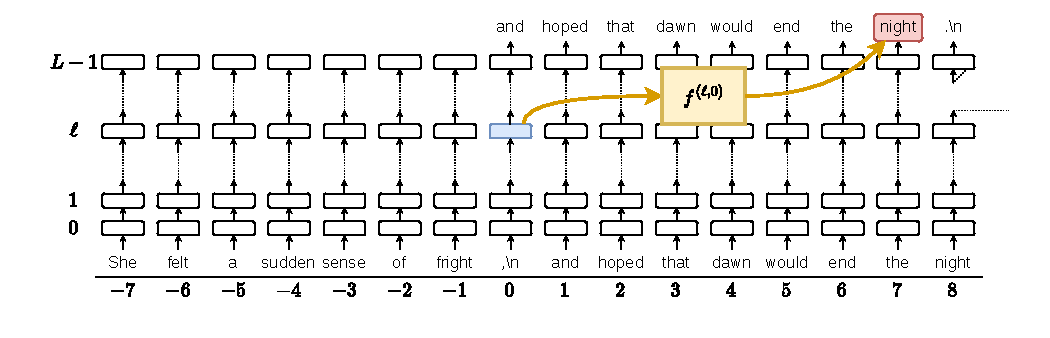
\includegraphics[width=\linewidth]{media/diagrams/probe-diagram.pdf}
    \caption{A linear probe $f^{(\ell,0)}$ trained to predict the rhyming token from
    activations at the newline position ($i=0$).}
    \label{fig:poem-diagram}
\end{figure}

\begin{figure*}[t]
    \centering
    \begin{subfigure}{0.325\linewidth}
        \centering
        \subcaption[]{Qwen3-32B (Top-5 Acc.)}
        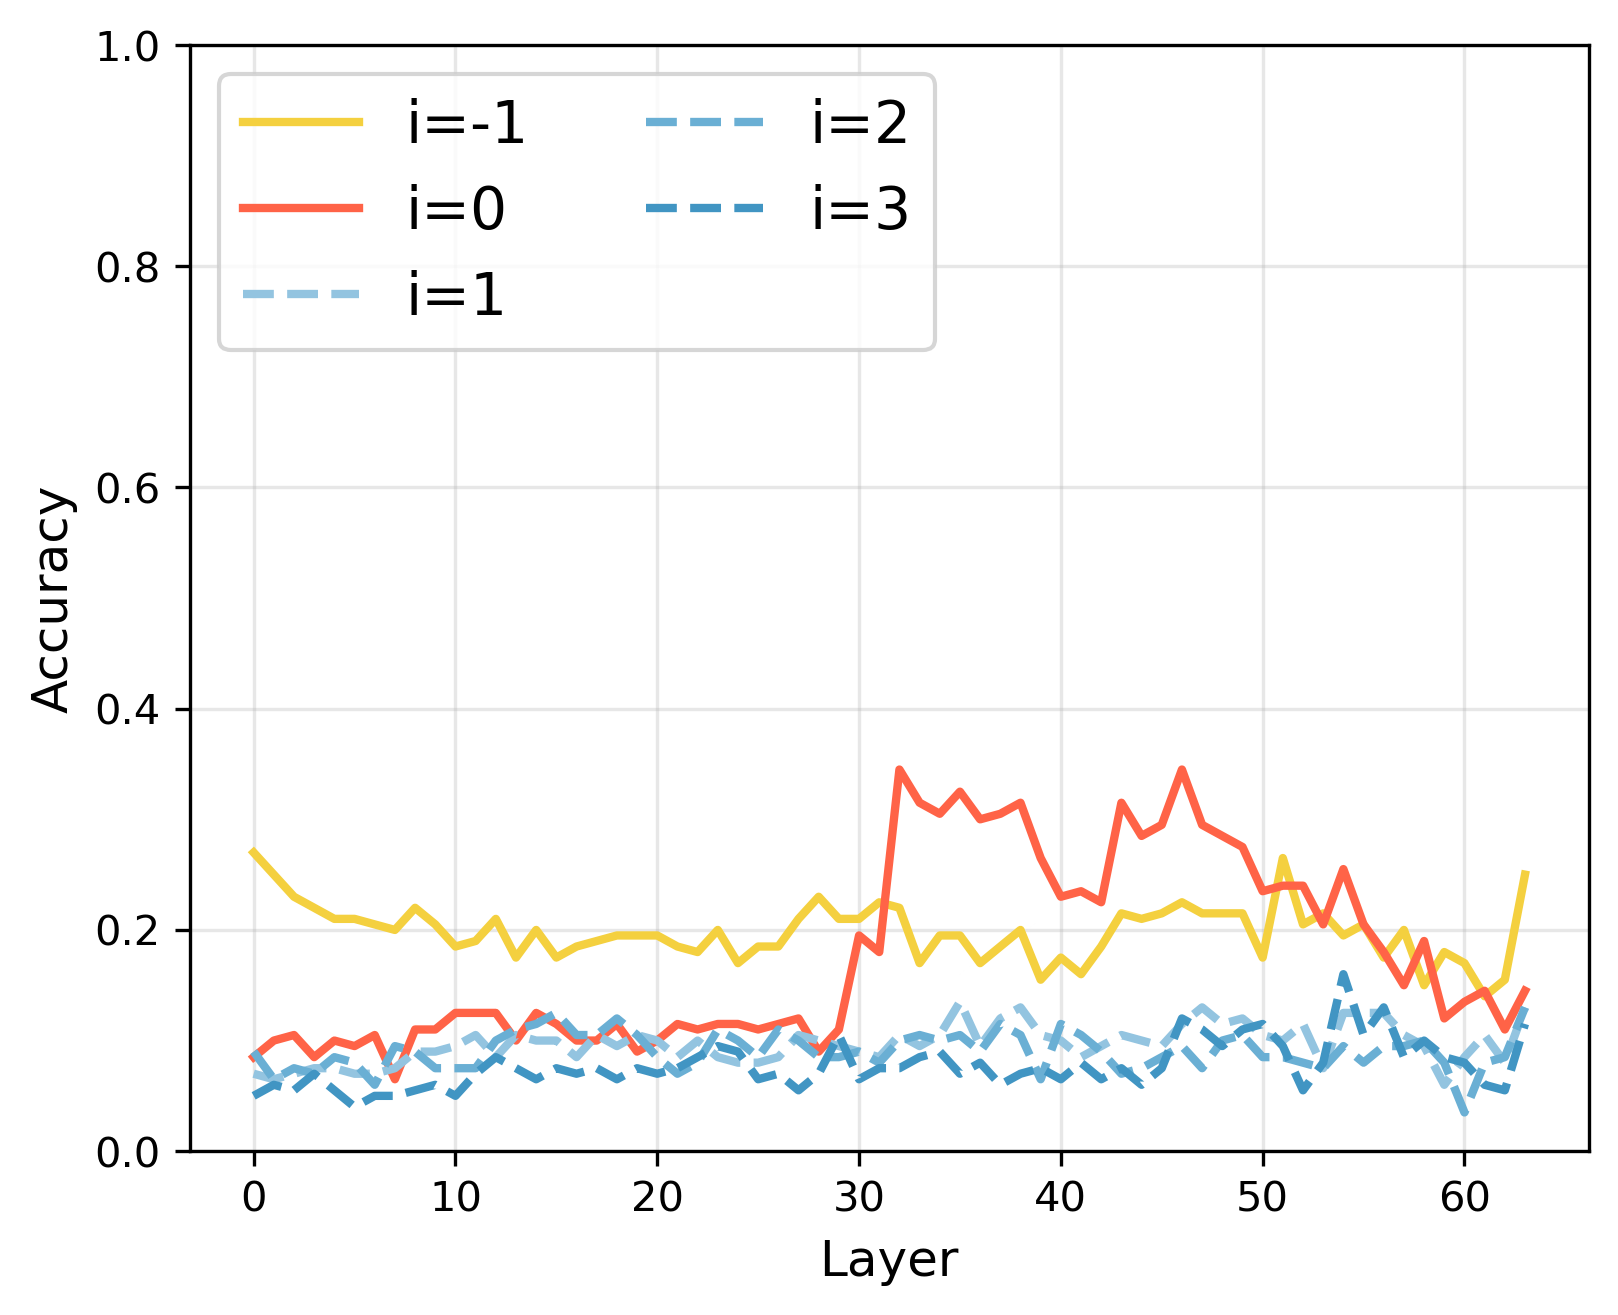
\includegraphics[width=\linewidth]{media/results-poem/qwen-top5.png}
    \end{subfigure}
    \begin{subfigure}{0.325\linewidth}
        \centering
        \subcaption[]{Gemma-3-27B (Top-5 Acc.)}
        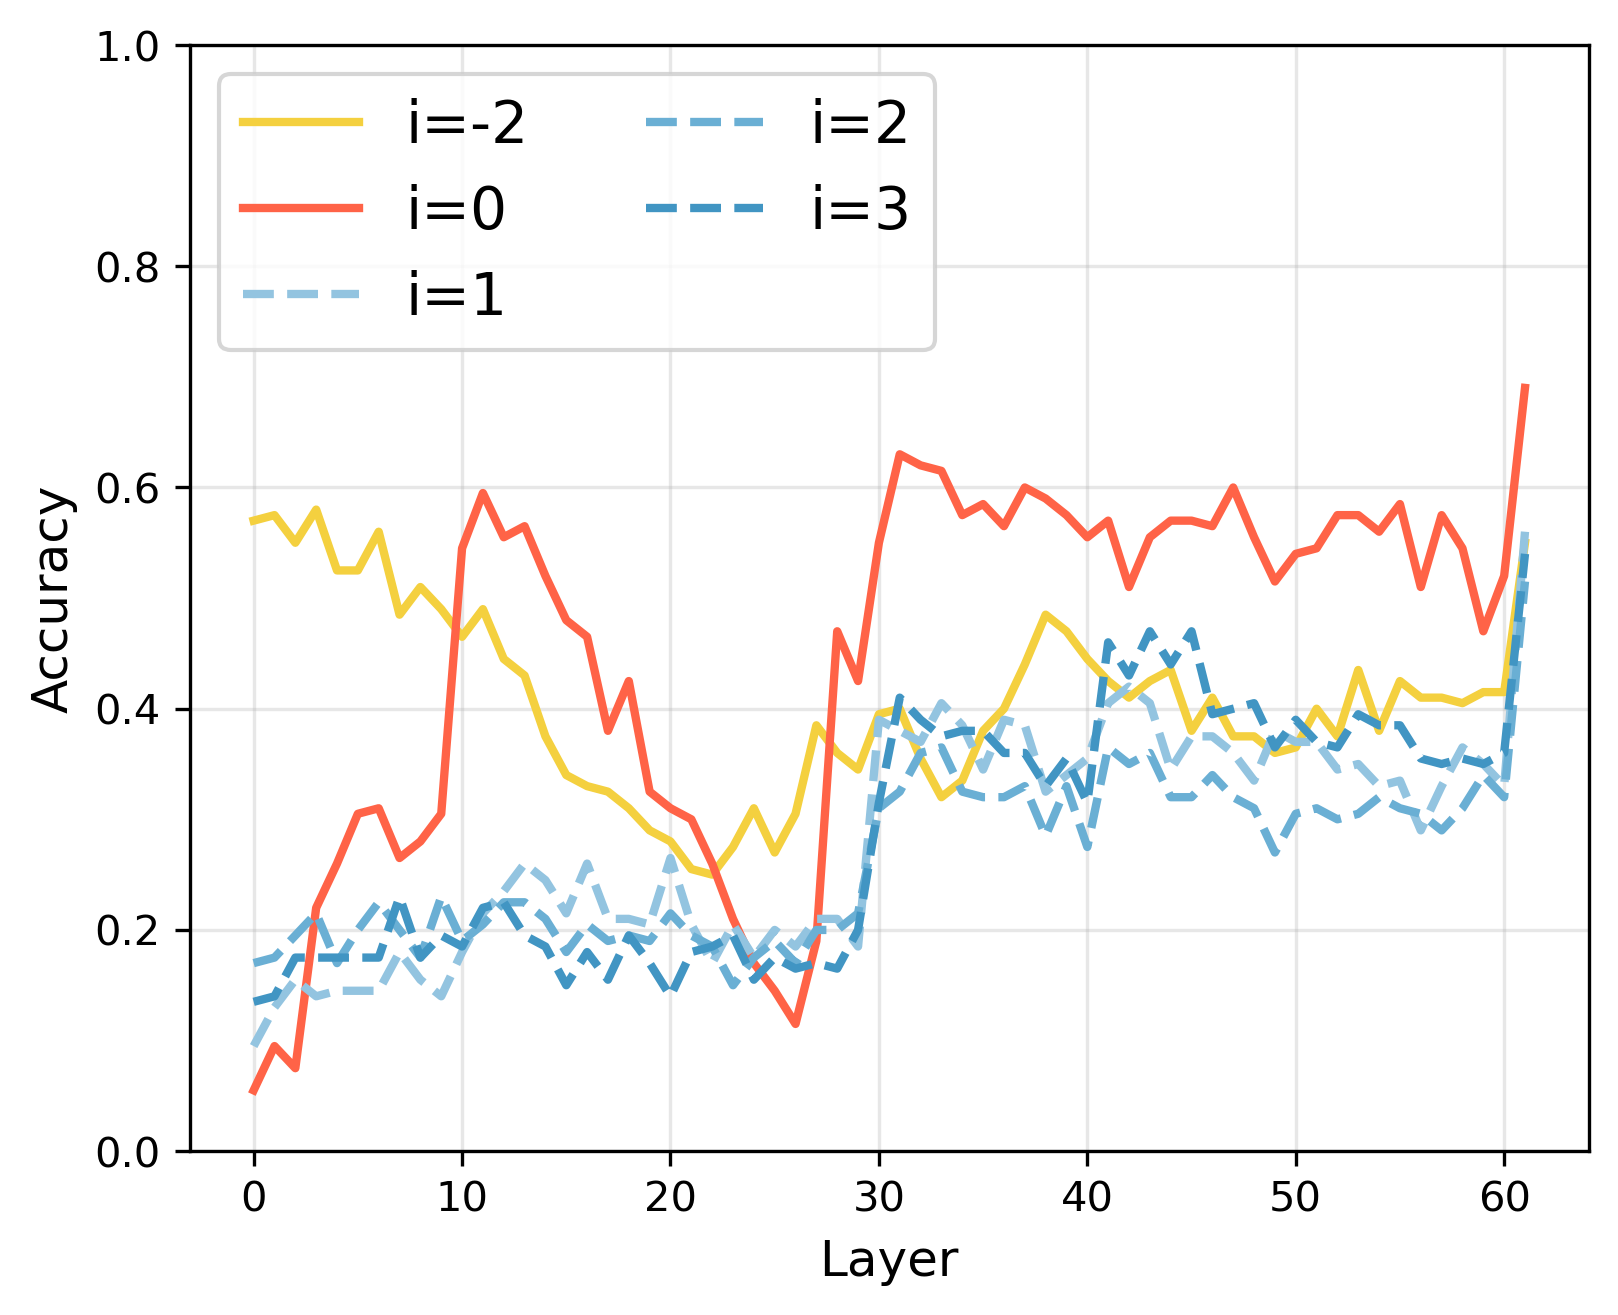
\includegraphics[width=\linewidth]{media/results-poem/gemma-top5.png}
    \end{subfigure}
    \begin{subfigure}{0.325\linewidth}
        \centering
        \subcaption[]{Llama-3.1-8B (Top-5 Acc.)}
        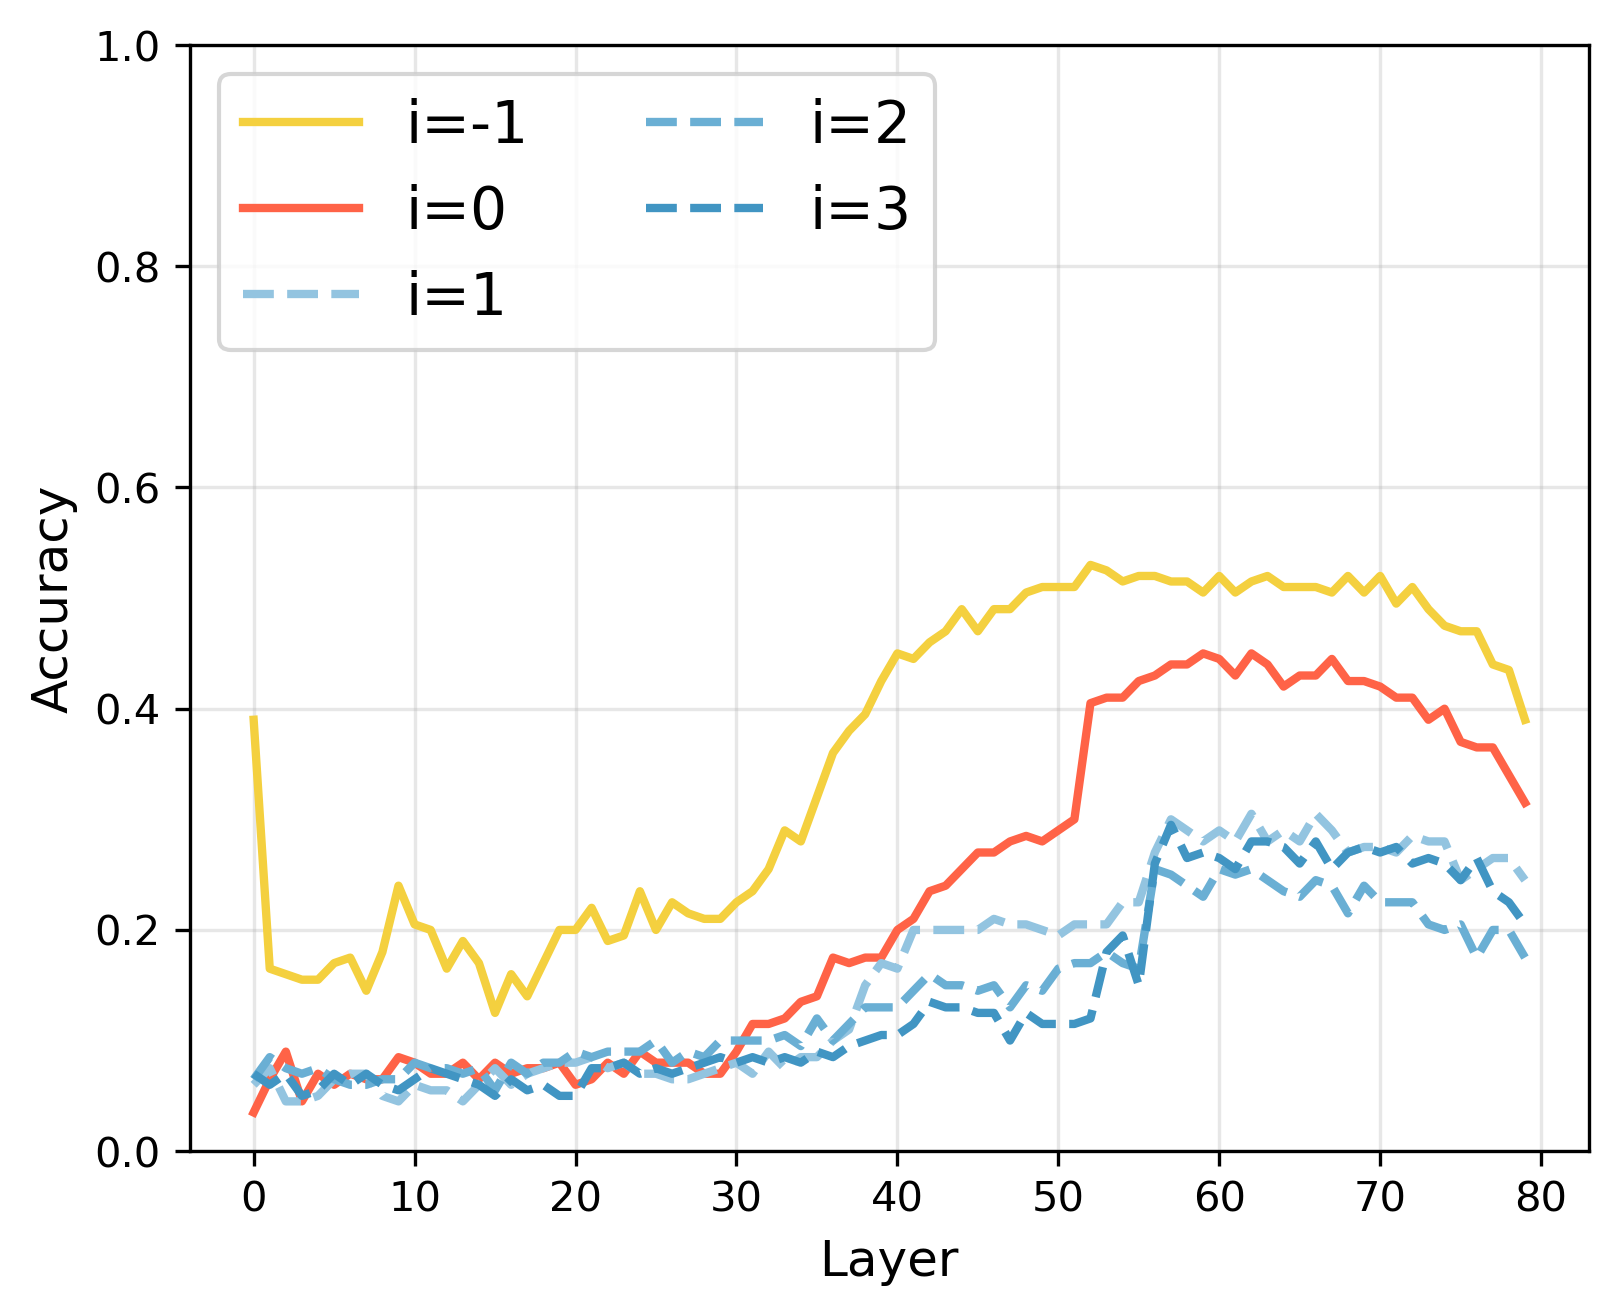
\includegraphics[width=\linewidth]{media/results-poem/llama-top5.png}
    \end{subfigure}
    \centering
    \begin{subfigure}{0.325\linewidth}
        \centering
        \subcaption[]{Qwen3-32B (Rhyme Acc.)}
        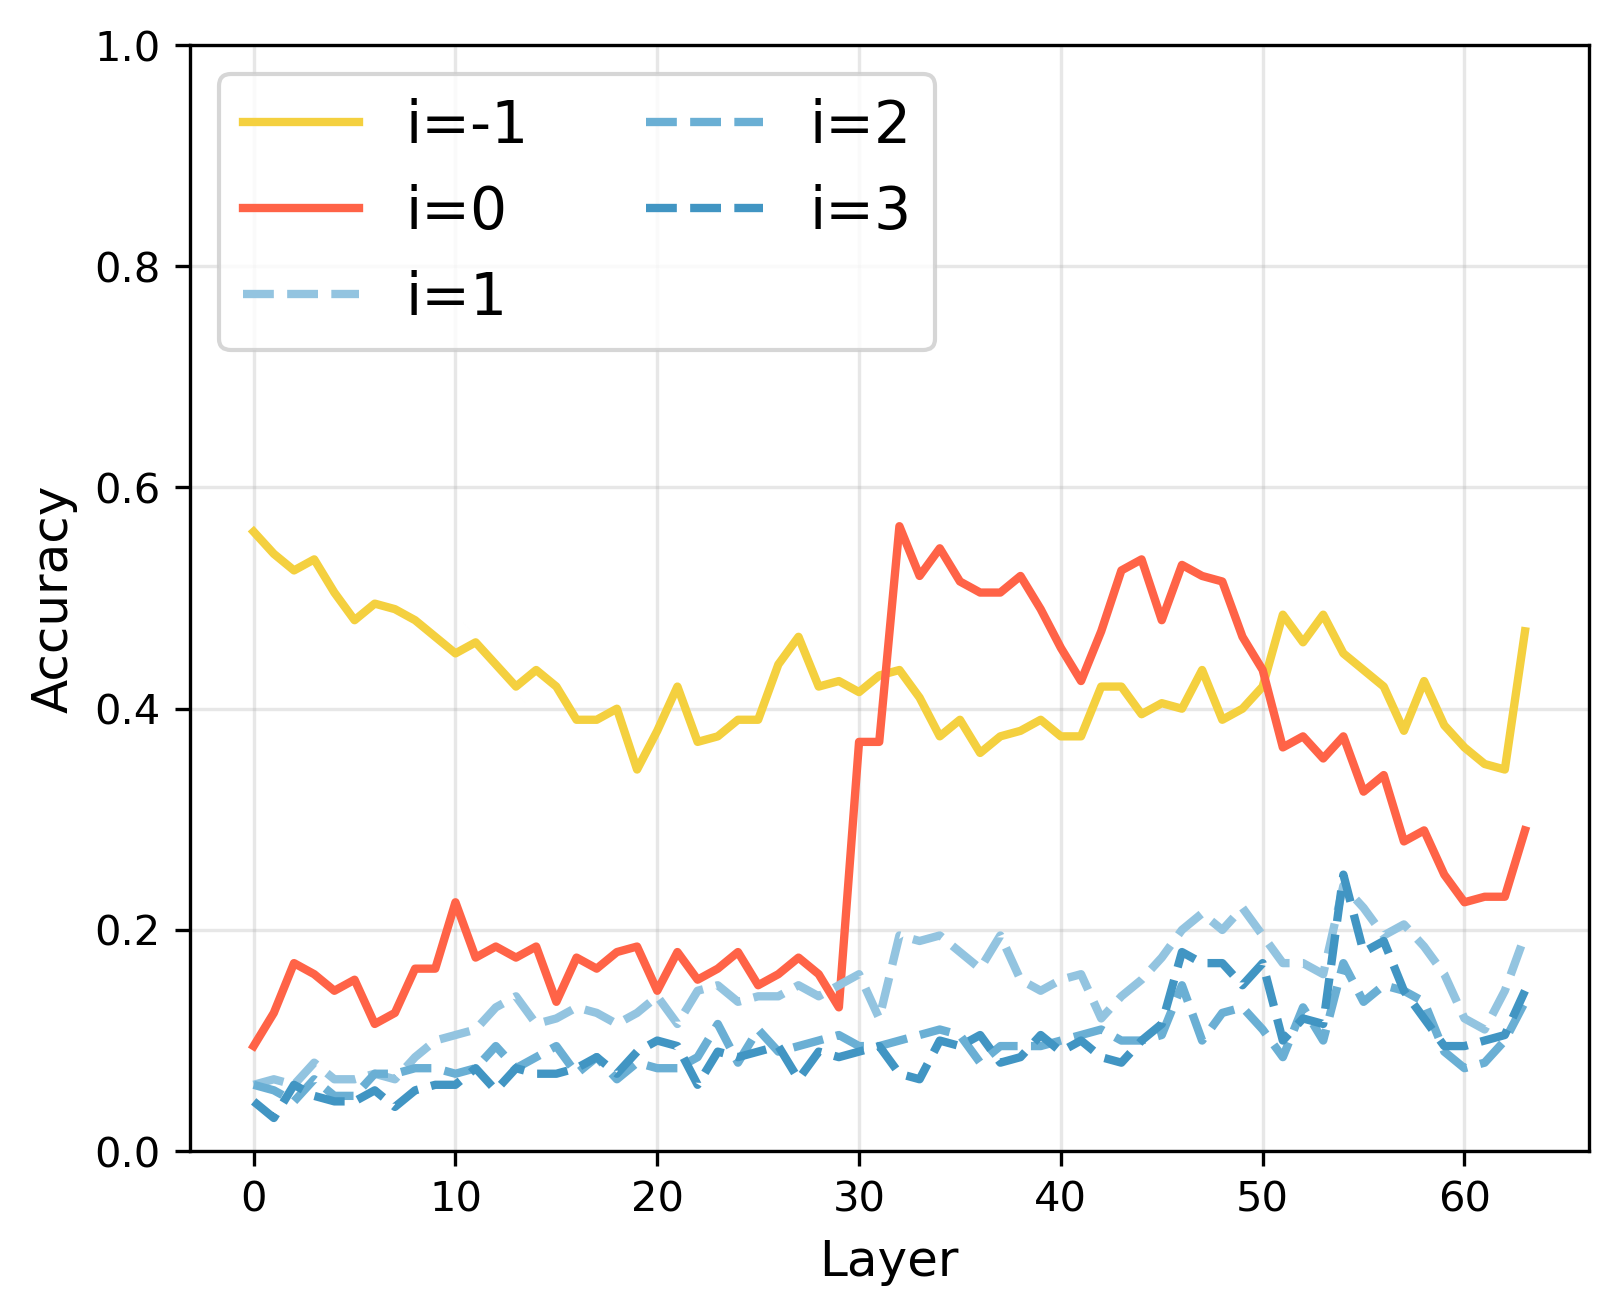
\includegraphics[width=\linewidth]{media/results-poem/qwen-rhyme1.png}
    \end{subfigure}
    \begin{subfigure}{0.325\linewidth}
        \centering
        \subcaption[]{Gemma-3-27B (Rhyme Acc.)}
        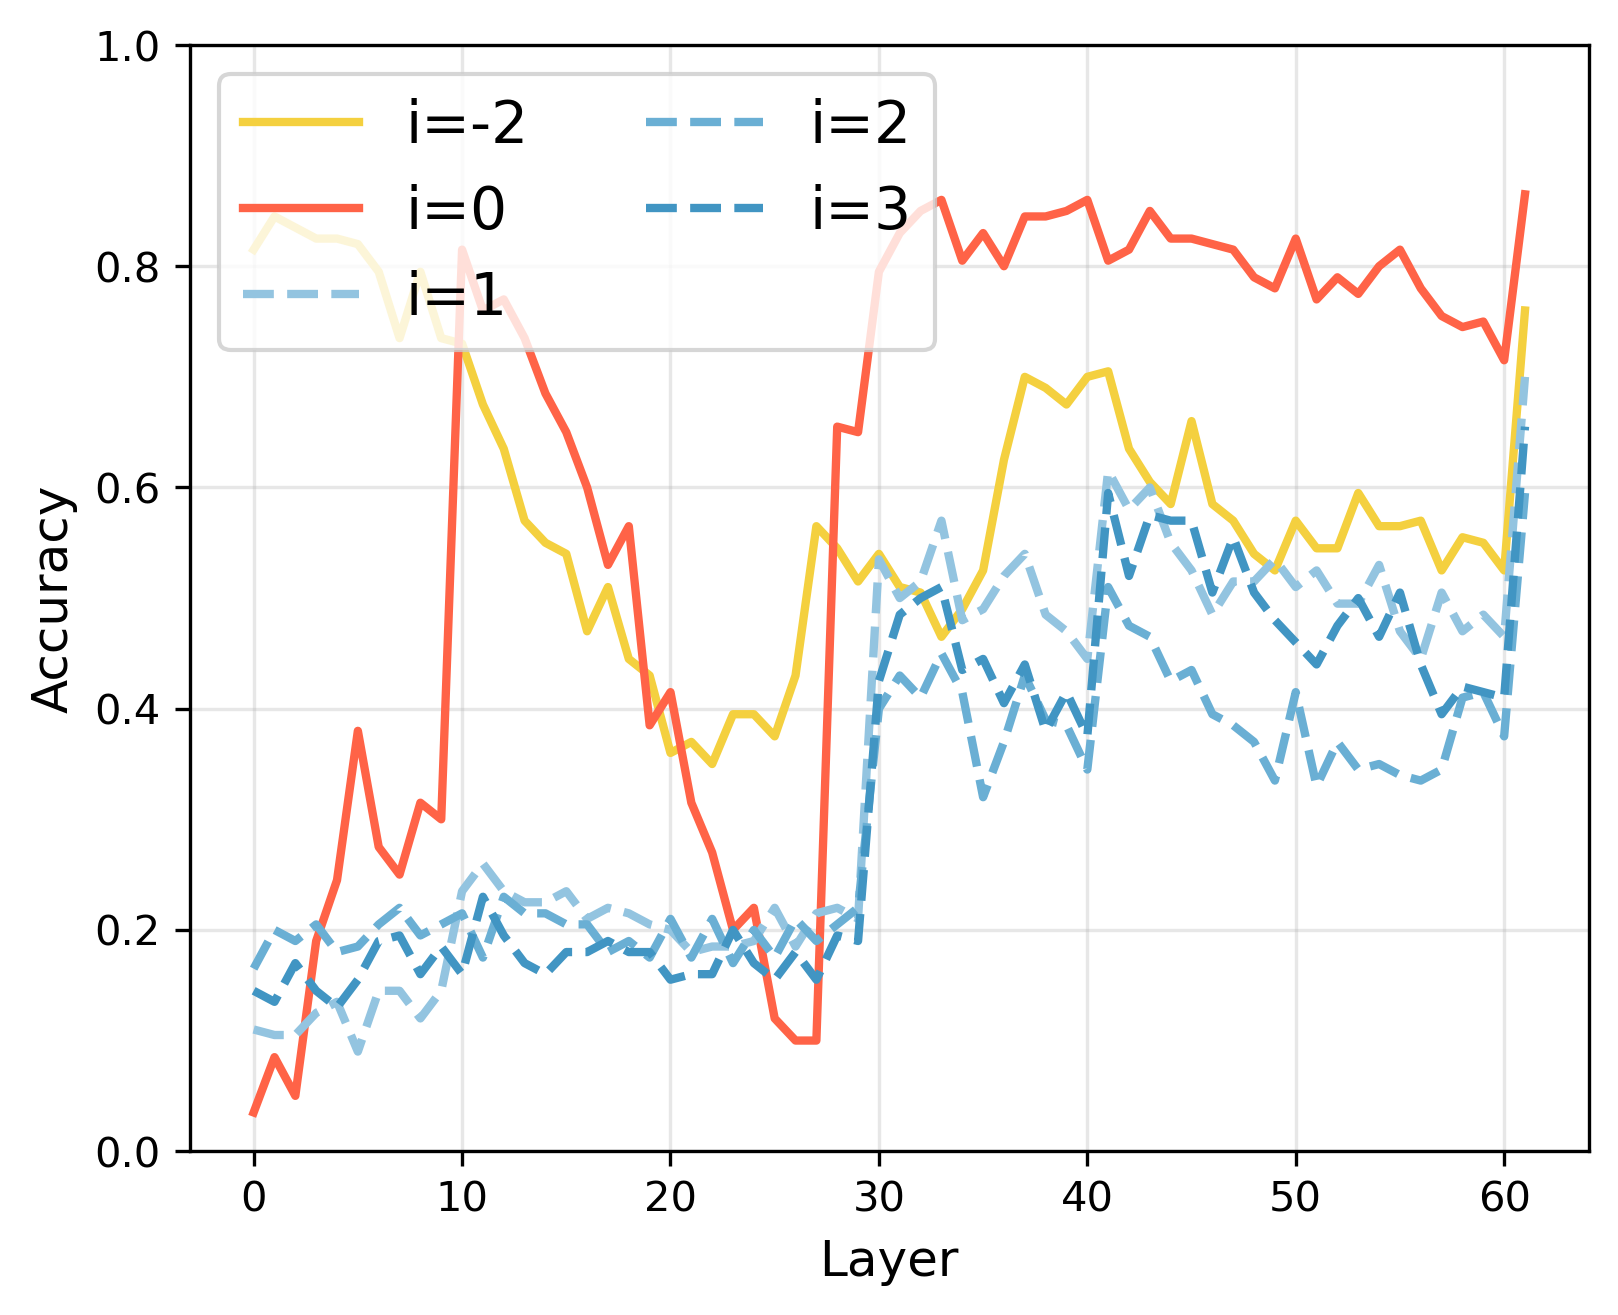
\includegraphics[width=\linewidth]{media/results-poem/gemma-rhyme1.png}
    \end{subfigure}
    \begin{subfigure}{0.325\linewidth}
        \centering
        \subcaption[]{Llama-3.1-8B (Rhyme Acc.)}
        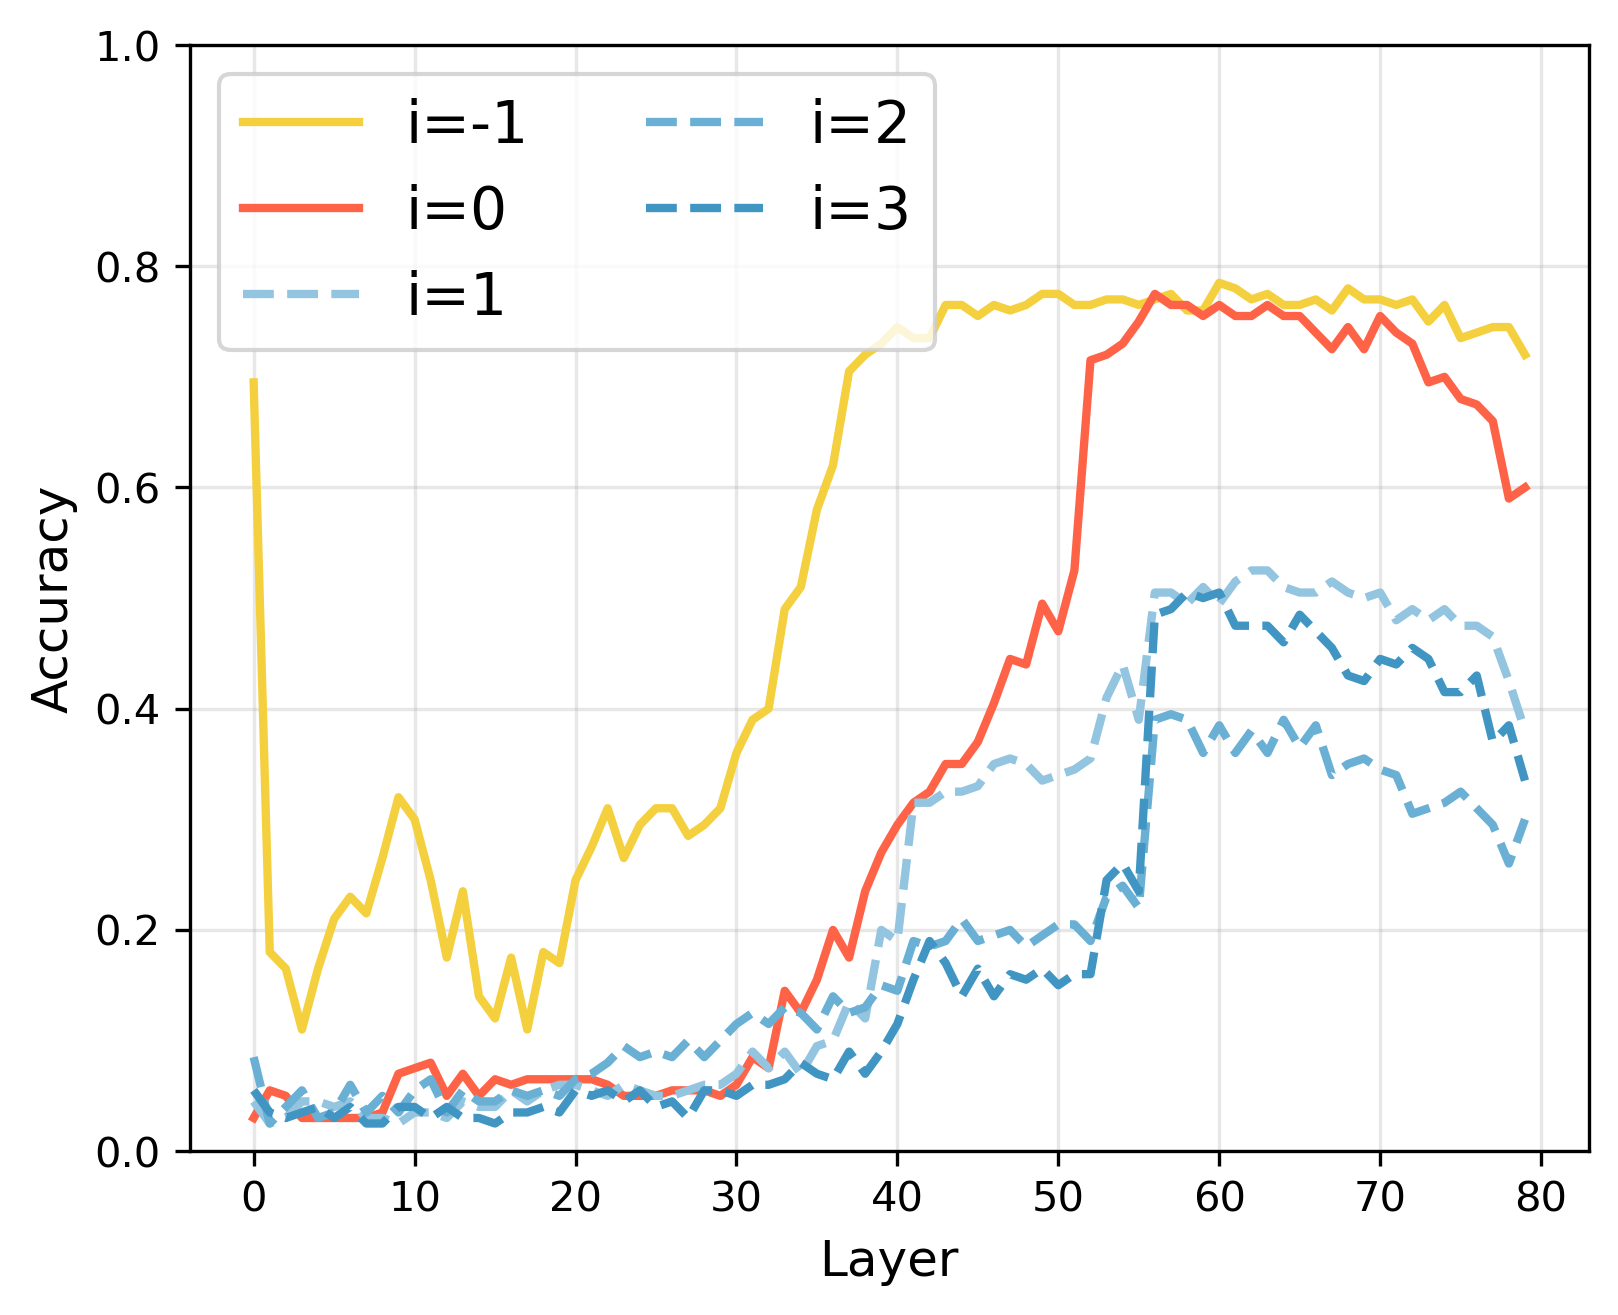
\includegraphics[width=\linewidth]{media/results-poem/llama-rhyme1.png}
    \end{subfigure}
    \caption{Top-5 and rhyme accuracy of linear probes trained to predict $r_2$ from hidden states at various layers and positions. Probes at the last word ($i\leq-1$) and newline ($i=0$) positions substantially outperform probes at subsequent generated positions ($i>0$), indicating that rhyme-relevant information is selectively concentrated at these structural positions.}
    \label{fig:poem-results}
\end{figure*}

First, we observe much higher accuracies probing to predict $r_2$ compared to general text.
On average, the generated $r_2$ is 8 tokens ahead of the newline token (the last context token), and we observe much greater accuracy for the $i=0$ probes compared to the $k=8$ probes on general text.
This suggests models selectively construct planning-compatible representations in response to the structural demands of rhyming couplet generation.

More significantly, we find evidence that these representations are concentrated in the last word and newline positions in certain layers (Figure~\ref{fig:poem-results}). This is demonstrated by the large differences in accuracy from the $i\leq0$ probes compared to the $i>0$ probes, which contradicts the pattern found while probing in general text that increasing look-ahead distance decreases probe accuracy.

Notably, probes trained on activations at the last word position all peak in accuracy early and decrease later, consistent with lexical identity of $r_1$ being encoded from the earliest layers.

However, it is nontrivial that probes trained at the newline position also do perform well, hinting at the possibility of latent planning occurring at the newline token. Notably, probes trained at both positions vastly differ in the shape of their accuracy curves between layers compared to probes at $i>0$, which seem to follow a similar shape throughout. This suggests that the newline and last word tokens undergo qualitatively different computations across layers, consistent with these positions playing a specialized role in encoding rhyme-relevant information rather than passively accumulating context like later positions.

Replicating this experiment on smaller Qwen, Gemma, and Llama models reveals these planning-compatible representations at the newline token emerge with scale. For each model, we record the largest accuracy gap across layers between probes trained at the newline token and probes trained at the next token. We find that this accuracy gap increases significantly with scale (Figure~\ref{fig:poem-scaling}), suggesting that planning-compatible representations are an emergent property.

\begin{figure*}[t]
    \centering
    \begin{subfigure}{0.49\linewidth}
        \centering
        
\includegraphics[width=\linewidth]{media/results-poem/scaling-top5.png}
        \subcaption[]{Top-5 Accuracy Difference}
    \end{subfigure}
    \begin{subfigure}{0.49\linewidth}
        \centering
        
\includegraphics[width=\linewidth]{media/results-poem/scaling-rhyme1.png}
        \subcaption[]{Rhyme Accuracy Difference}
    \end{subfigure}
    \caption{Maximum accuracy gap across layers between probes at the newline ($i=0$) and the first generated position ($i=1$), plotted against model size. The gap increases with scale across all three model families, suggesting that planning-compatible representations at the newline are an emergent property of larger models.}
    \label{fig:poem-scaling}
\end{figure*}


\subsection{Discussion and limitations of probing}
\label{sec:probe-discussion}

The probing results reveal substantial cross-model and cross-scale diversity in planning-compatible representations at both the last word and newline positions. However, several alternative explanations warrant consideration.

First, the elevated newline probe accuracy could reflect passive attention accumulation rather than active planning: if models attend strongly from the newline to the rhyme word in the first line, the newline hidden state will encode rhyme-relevant information even without any downstream computation reading it out during generation. Also, rhyme accuracy as a metric is imperfect, as the CMU Pronouncing Dictionary does not capture all valid rhymes, potentially underestimating probe performance inconsistently across rhyme families. Additionally, though we prompted Claude to generate couplets with diverse subjects and rhyme schemes, the resulting dataset may still carry nontrivial distributional biases that could inflate probe accuracy in ways difficult to detect or control for.

These considerations highlight two fundamental limitations of probing as a method. First, high probe accuracy establishes that rhyme-relevant information is linearly decodable at a position, but cannot establish that this information causally drives generation. Second, probe accuracy is sensitive to the distribution of the training data, meaning results could partially reflect dataset artifacts rather than genuine planning representations.

Activation patching addresses both limitations directly: by intervening on specific hidden states during generation and measuring the causal effect on output, it neither requires a probe training distribution nor conflates passive encoding with active deployment. We turn to activation patching in the next section to resolve these ambiguities.



\section{Patching for Causally Active Planning Sites}
\label{sec:patching}

\begin{figure}[t]
    \centering
    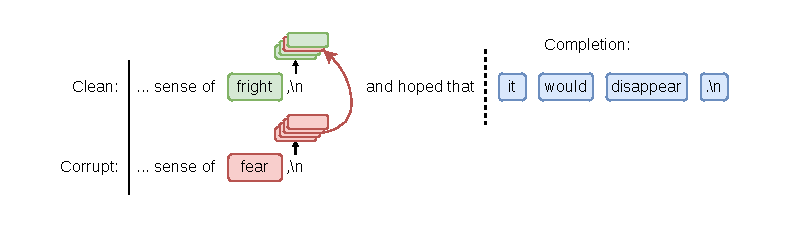
\includegraphics[width=\linewidth]{media/diagrams/patch2-diagram.pdf}
    \caption{Activation patching: the hidden state $\mathbf{h}_{\ell,i}$ from a corrupted run is substituted into the clean run's forward pass at position $i$ and layer $\ell$. A successful patch redirects generation toward the corrupted rhyme family, providing causal evidence that $(i,\ell)$ is a planning site.}
    \label{fig:patch-diagram}
\end{figure}

While probing reveals that future token information is encoded in hidden states, it does not establish that this information is causally used by the model. In this section, we further investigate latent planning in rhyming couplet generation by employing intervention methods to test for causal influence directly. Given a prompt $\mathbf{x}^{(c)}$ whose first line naturally leads to a clean rhyme family $\mathcal{R}^{(c)}$, we intervene on the model's activations at various positions and investigate whether the generation of the second line shifts toward a different corrupted rhyme family $\mathcal{R}^{(r)}$. A successful intervention on a specific layer $\ell$ and position $i$ provides causal evidence that information at $\mathbf{h}_{\ell, i}$ is causally involved in the model's latent planning downstream.

\begin{figure*}[t]
    \centering
    \begin{subfigure}{0.32\linewidth}
        \centering
        
\includegraphics[width=\linewidth]{media/results-patching/patching_qwen3_32b.png}
        \caption{Qwen3-32B.}
        \label{fig:patch-qwen}
    \end{subfigure}
    \hfill
    \begin{subfigure}{0.32\linewidth}
        \centering
        
\includegraphics[width=\linewidth]{media/results-patching/patching_gemma3_27b.png}
        \caption{Gemma-3-27B.}
        \label{fig:patch-gemma}
    \end{subfigure}
    \hfill
    \begin{subfigure}{0.32\linewidth}
        \centering
        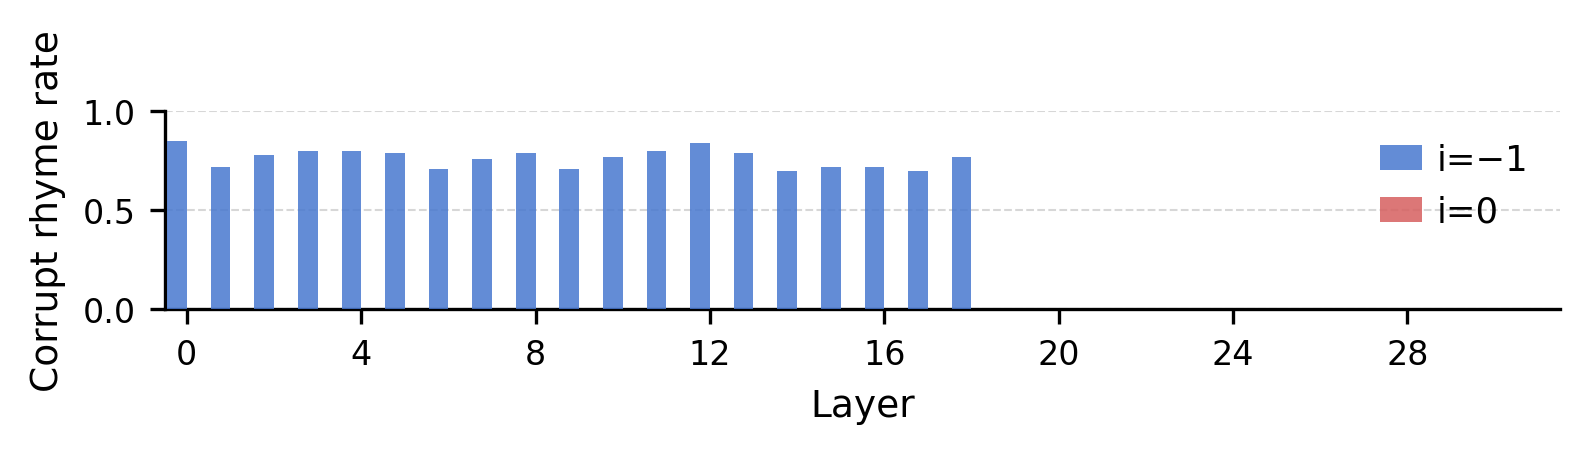
\includegraphics[width=\linewidth]{media/results-patching/patching_llama_8b.png}
        \caption{Llama-3.1-8B.}
        \label{fig:patch-llama}
    \end{subfigure}
    \caption{Per-layer activation patching at the last word token and newline ($i=0$) for the largest model in each family. Full results for all model sizes are in Appendix~\ref{sec:additional-patching-details}.}
    \label{fig:patch-results}
\end{figure*}

We apply activation patching at two positions: the last word token (position $i=-1$ in Qwen3 and Llama-3, $i=-2$ in Gemma-3 due to its tokenization of the line-ending comma; see Appendix~\ref{sec:model-config}) and the newline token ($i=0$), sweeping across all layers individually. For each layer, we report the corrupt rhyme rate averaged over 20 prompt pairs. Figure~\ref{fig:patch-results} shows results for the largest model in each family.

In Gemma-3-27B (Figure~\ref{fig:patch-gemma}), last-word patching is highly effective in early layers but drops sharply around layer 30, while newline patching rises simultaneously to a peak corrupt rhyme rate of ${\sim}0.63$ at layers 33--35. This crossover, which we term the \textit{representational handoff}, is the mechanistic signature of \textit{planning site formation}: the causal locus migrates from the last word token to the newline, which becomes the primary read-out site for the phonological constraint. In contrast, Qwen3-32B (Figure~\ref{fig:patch-qwen}) and Llama-3.1-8B (Figure~\ref{fig:patch-llama}) show uniformly high last-word patching and near-zero newline patching across all layers, indicating that no such migration occurs. These models condition on the last word token throughout generation. Per-layer results for all model sizes within each family are provided in Appendix~\ref{sec:additional-patching-details}.

\subsection{Localizing the Handoff to a Sparse Set of Attention Heads}
\label{sec:head-patching}

\begin{figure*}[!t]
    \centering
    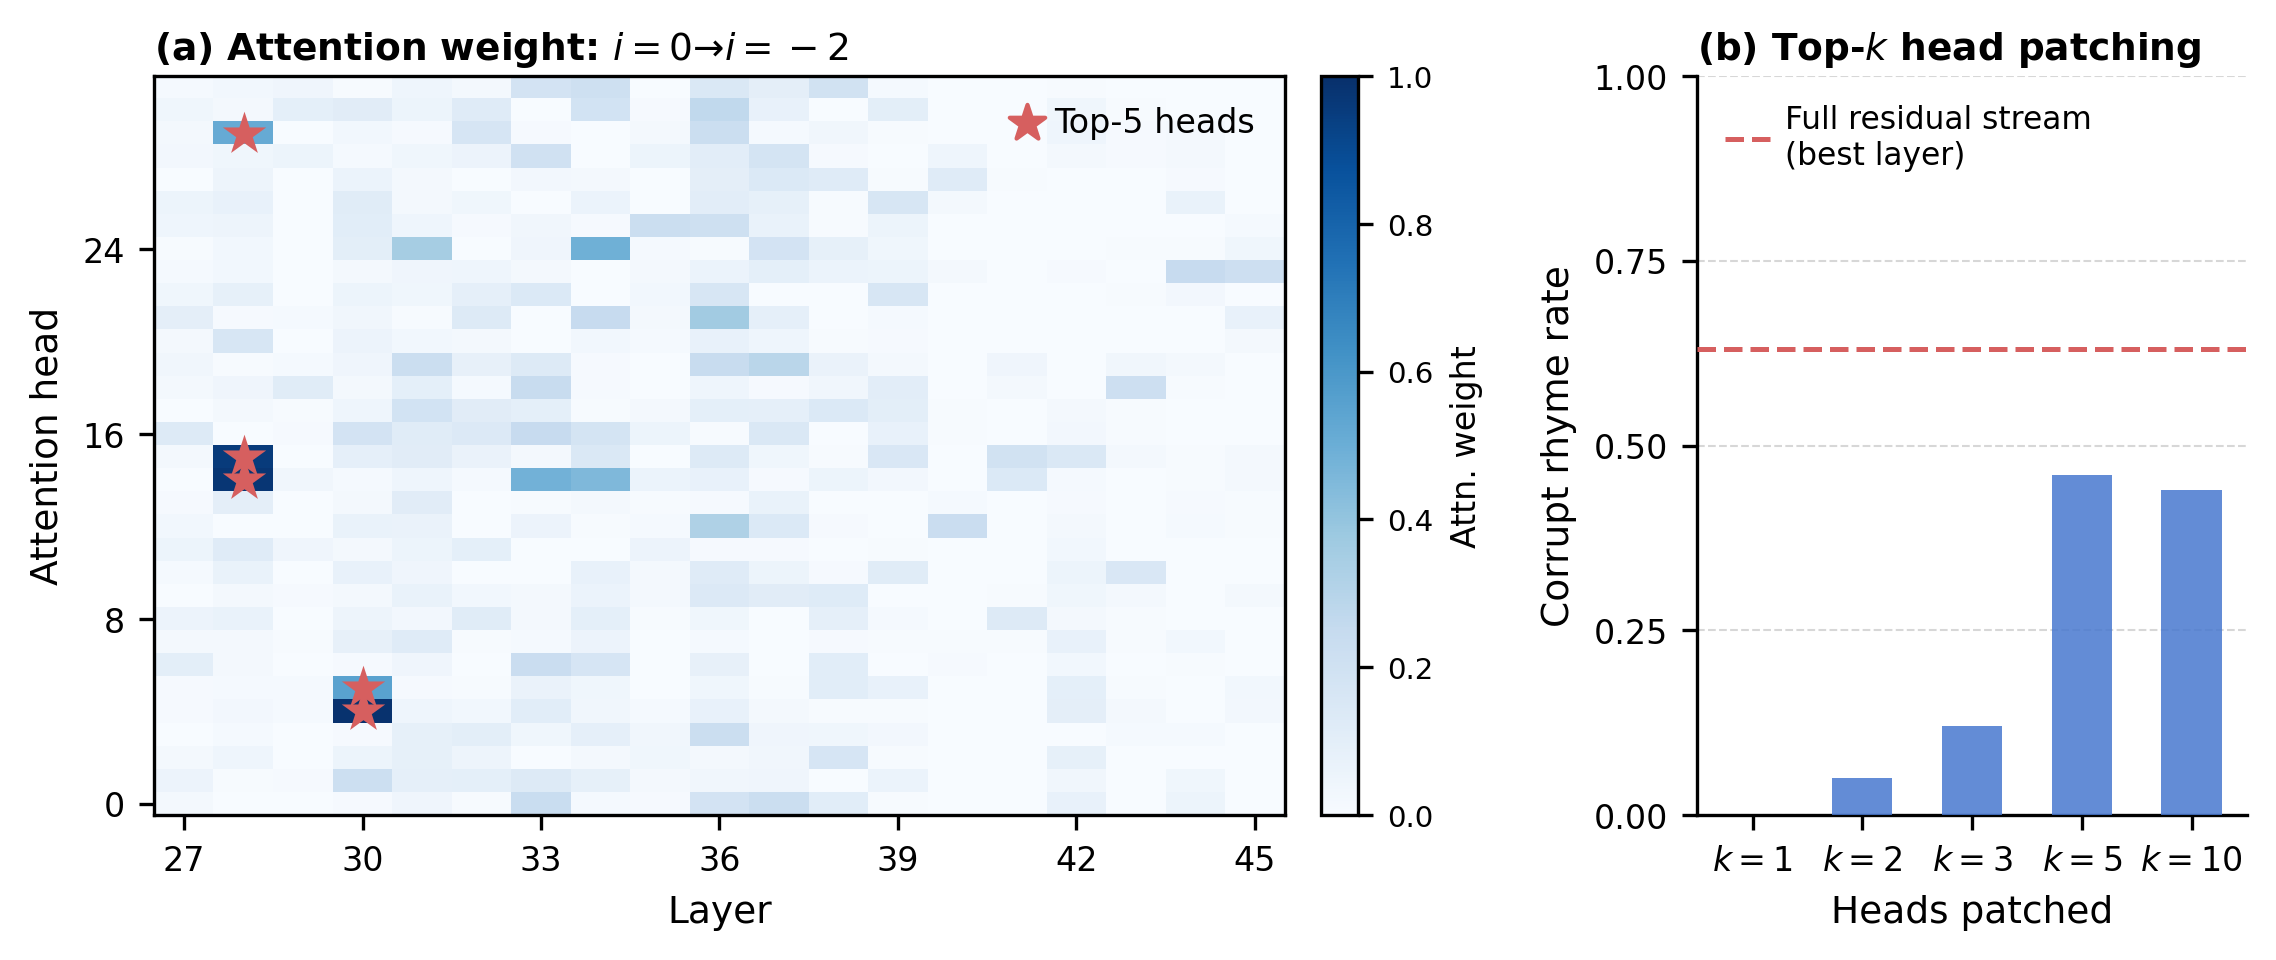
\includegraphics[width=\linewidth]{media/results-patching/topk_head_patching.png}
    \caption{Localizing the planning site handoff in Gemma-3-27B to a sparse set of attention heads. \textbf{(a)} Attention weight from the newline token ($i=0$) to the last word token ($i=-2$) across heads in layers 27--45. Red stars mark the top-5 heads by attention weight. \textbf{(b)} Corrupt rhyme rate when patching the top-$k$ highest-attending heads simultaneously at the newline. The dashed line shows the reference level from full residual-stream patching at the best single layer (${\sim}0.63$).}
    \label{fig:topk-heads}
\end{figure*}

Having established that the planning site forms at the newline token in Gemma-3-27B, we ask whether the information routing handoff can be attributed to a small, identifiable set of attention heads. Single-head patching at the newline (replacing one head's output at a time within the planning layer range, layers 27--45) produced no measurable signal for any individual head, suggesting the representation is not localized to a single circuit element. Exhaustive combinatorial search over head subsets is computationally infeasible, so we instead use attention weights as a proxy for which heads are most likely to route rhyme information from the last word token to the newline.

Specifically, we extract the attention weight from the newline token ($i=0$) to the last word token ($i=-2$) for each head in layers 27--45 of both clean and corrupt forward passes, and rank heads by this weight. Figure~\ref{fig:topk-heads}a shows the resulting heatmap: attention to $i=-2$ is highly concentrated: three heads attend almost exclusively to the last word token from the newline, namely layer 30 head 4 (weight ${\approx}0.99$), layer 28 head 14 (${\approx}0.97$), and layer 28 head 15 (${\approx}0.95$). A second cluster of heads in layers 28--36 shows moderate attention weights (0.35--0.55).

We then patch the top-$k$ heads by attention weight simultaneously, replacing their outputs at the newline position with those from the corrupt forward pass, and measure the resulting corrupt rhyme rate. Figure~\ref{fig:topk-heads}b shows that $k=1,2,3$ produce near-zero corrupt rhyme rates (0.00, 0.05, and 0.12, respectively), indicating that even the three highest-attending heads are individually and jointly insufficient to carry the full phonological signal. At $k=5$, the corrupt rhyme rate jumps to ${\sim}0.46$, comparable to the peak achieved by full residual stream patching at the best single layer (${\sim}0.63$, shown as a dashed reference). Adding further heads ($k=10$) does not improve the rate, which plateaus at ${\sim}0.44$.

These results reveal a sparse but distributed implementation of the handoff: a set of five attention heads spanning layers 28--34 collectively account for the bulk of the rhyme information routed to the newline, while individual heads or smaller subsets are insufficient. The top five heads by attention weight are (layer 30, head 4), (layer 28, head 14), (layer 28, head 15), (layer 30, head 5), and (layer 28, head 29). We also verified that patching top-$k$ MLP layer outputs at the same position yields zero corrupt rhyme rate for all $k$, confirming that the handoff is mediated by attention rather than feed-forward computation.


\section{Conclusion}

We introduced the notion of \textit{planning site formation} and investigated it across three model families and more than ten model sizes using linear probing and activation patching. Our central finding is a categorical dissociation: Gemma-3-27B is the only model that forms a causally active planning site at the newline token, doing so via an information routing handoff in which the causal locus migrates from the last word token to the newline around layer 30. Every other tested model (all Qwen3 sizes from 0.6B to 32B, all Llama-3 sizes from 1B to 8B, and all smaller Gemma-3 models) conditions on the last word token throughout generation.

The Qwen3 family provides the paper's sharpest methodological lesson. Probing reveals strong, scale-dependent planning-compatible representations at the newline across all Qwen3 sizes, yet activation patching shows near-zero causal effect at every scale. Planning-compatible representations and causally active planning sites are dissociable: probe signal is not sufficient evidence of a planning site, and activation patching is required to establish causal relevance.

Beyond the layer-level analysis, we localize the handoff in Gemma-3-27B to a sparse set of five attention heads in layers 28--34, identified via attention weight ranking followed by simultaneous head patching. Patching these five heads at the newline recovers ${\sim}73\%$ of the effect achievable by full residual-stream patching, while single-head patching and MLP patching produce no effect. This circuit-level specificity, with a handful of attention heads implementing a representational handoff, suggests that planning site formation, when it occurs, is a structured computational phenomenon rather than a diffuse property of many model components.

Our activation patching approach requires no transcoder training and far less data than steering vector approaches, making it scalable to large models across many architectures. The results, however, also surface important open questions and limitations that future work should address.

First, our analysis is limited to three model families on a single structured generation task (rhyming couplets). Extending the methodology to prose generation, code completion, and multi-step reasoning tasks would test whether the representational handoff is a general planning primitive or a narrow phonological phenomenon. Second, while we localize the Gemma-3-27B handoff to five attention heads, we do not yet trace the full information-flow circuit. Path patching~\citep{goldowsky2023localizing} from the last word token through these heads to the downstream generation would clarify whether the circuit is feedforward or involves recursive refinement. Third, the absence of the handoff in all Qwen3 and Llama-3 models despite strong probe signal raises a question about what distinguishes Gemma-3-27B architecturally or by training. Finally, causal scrubbing~\citep{chan2022causal} or activation steering experiments targeting the planning heads would help distinguish whether the planning representation at the newline is genuinely read during generation or exerts influence only when artificially inserted via patching.


\bibliography{references}
\bibliographystyle{icml2026}

\appendix

\section{Model Configurations}
\label{sec:model-config}
For reference, we report details of the architectural differences between models.

\begin{table}[h]
\centering
\begin{tabular}{lccc}
\toprule
 & Qwen3-32B & Gemma-3-27B  & Llama-3.1-8B \\
\midrule
$|\mathcal V|$ & 151,936 & 262,208 & 128,256 \\
$d$            & 5,120   & 5,376   & 4,096  \\
$L$            & 64      & 62      & 32     \\
\bottomrule
\end{tabular}
\caption{Model architecture summary.}
\label{tab:models}
\end{table}

We also note important tokenization differences. Qwen and Llama treat \texttt{,\textbackslash n} as a single token, while Gemma treats
\texttt{,} and \texttt{\textbackslash n} as separate tokens.
This places the last word $r_1$ at position $-1$ in Qwen and Llama and position $-2$ in Gemma.

\begin{table}[h]
\centering
\small
\begin{tabular}{ccccc}
\toprule
 & $-2$ & $-1$ & $0$ & $1$ \\
\midrule
Qwen3   & \texttt{of}     & \texttt{fright} & \texttt{,\textbackslash n} & \texttt{and} \\
Llama-3 & \texttt{of}     & \texttt{fright} & \texttt{,\textbackslash n} & \texttt{and} \\
Gemma-3 & \texttt{fright} & \texttt{,}      & \texttt{\textbackslash n}  & \texttt{and} \\
\bottomrule
\end{tabular}
\caption{Tokenization of the line boundary across model families.}
\end{table}


\section{Additional Probing Results}
\label{sec:additional-probing-results}
For probing experiments, we also evaluated on top-1 accuracy. Note these are similar to the reported results, only scaled down.

\begin{figure}[H]
    \centering
    \begin{subfigure}{0.49\linewidth}
        \centering
        \subcaption[]{Qwen3-32B.}
        
\includegraphics[width=\linewidth]{media/results-probe/qwen-top1.png}
    \end{subfigure}
    \begin{subfigure}{0.49\linewidth}
        \centering
        \subcaption[]{Gemma-3-27B.}
        
\includegraphics[width=\linewidth]{media/results-probe/gemma-top1.png}
    \end{subfigure}
    \caption{Top-1 probe accuracy predicting $k$ tokens ahead in general text (Pile). Mirrors the top-5 pattern: accuracy degrades monotonically with $k$ and falls to unigram baseline by $k=8$.}
    \label{fig:appendix-probe}
\end{figure}

\begin{figure}[H]
    \centering
    \begin{subfigure}{0.49\linewidth}
        \centering
        \subcaption[]{Qwen3-32B}
        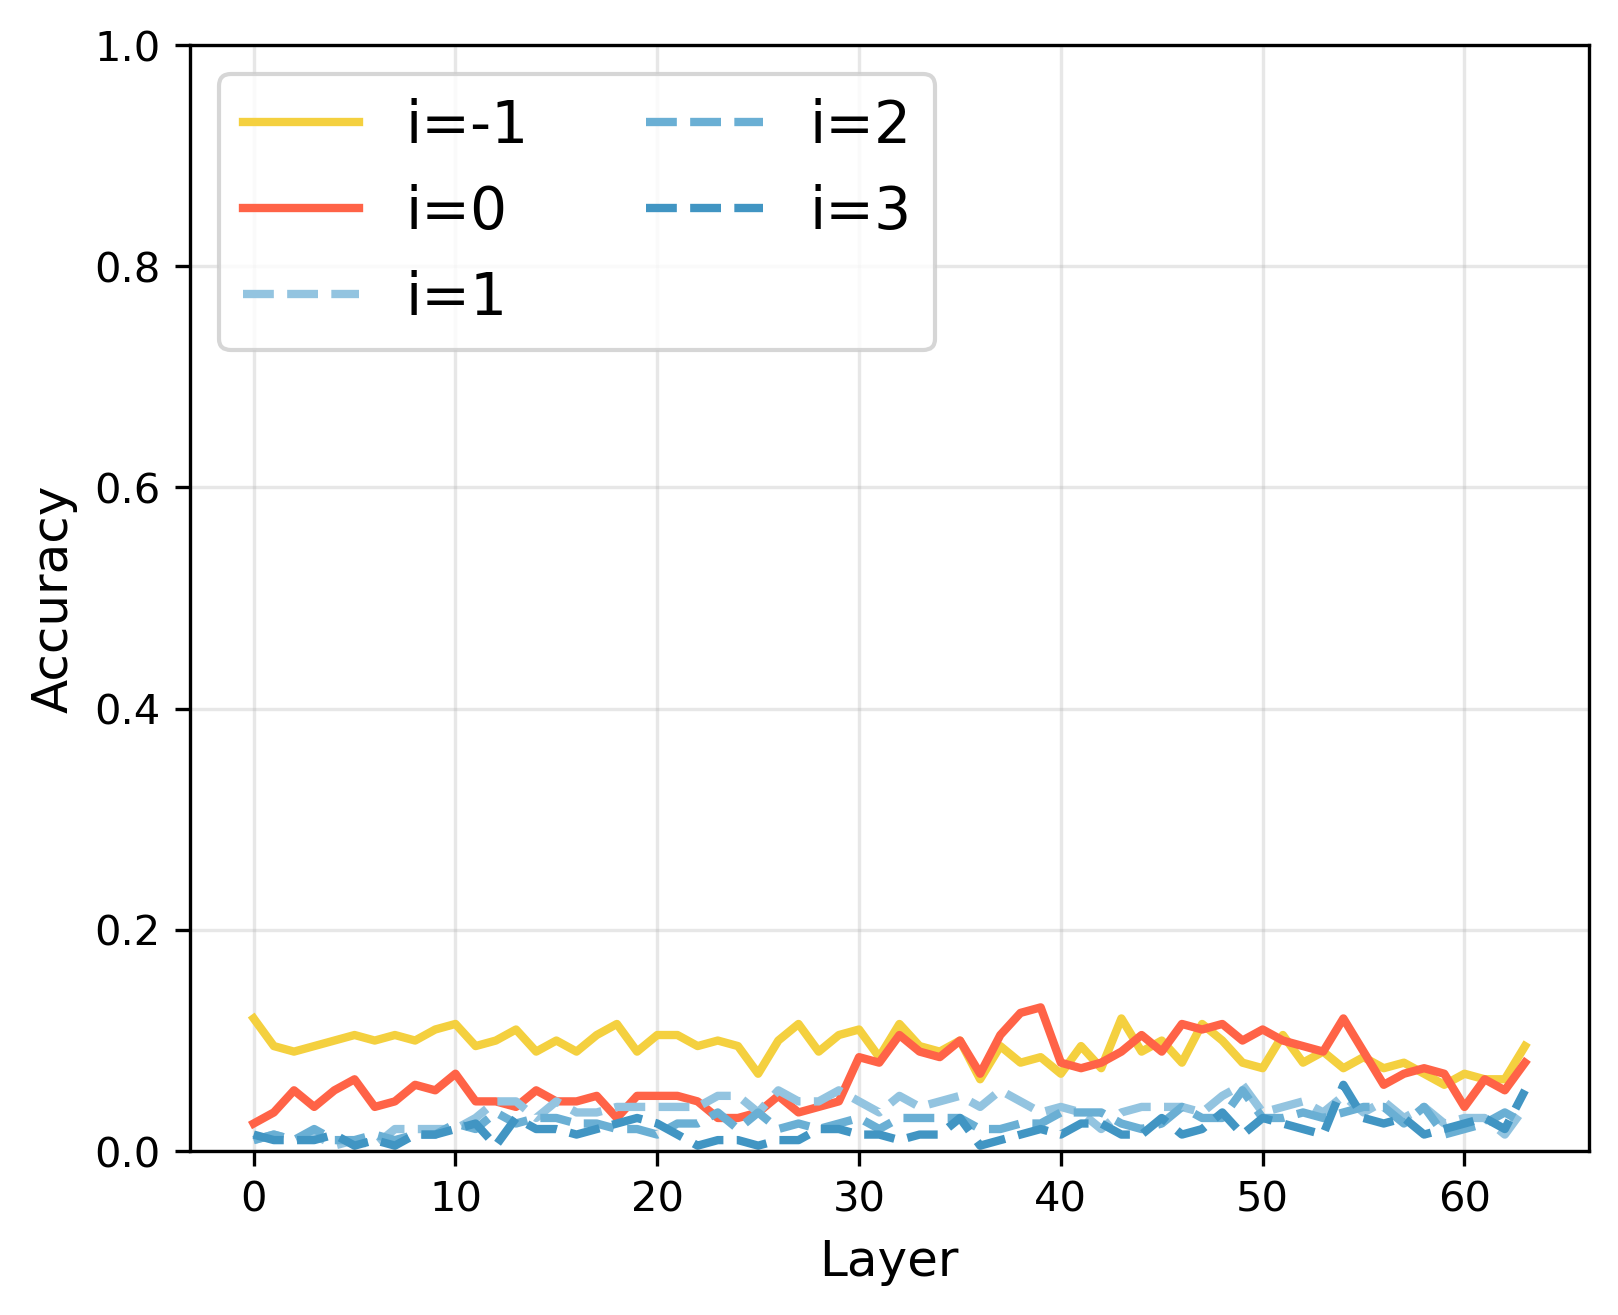
\includegraphics[width=\linewidth]{media/results-poem/qwen-top1.png}
    \end{subfigure}
    \begin{subfigure}{0.49\linewidth}
        \centering
        \subcaption[]{Gemma-3-27B}
        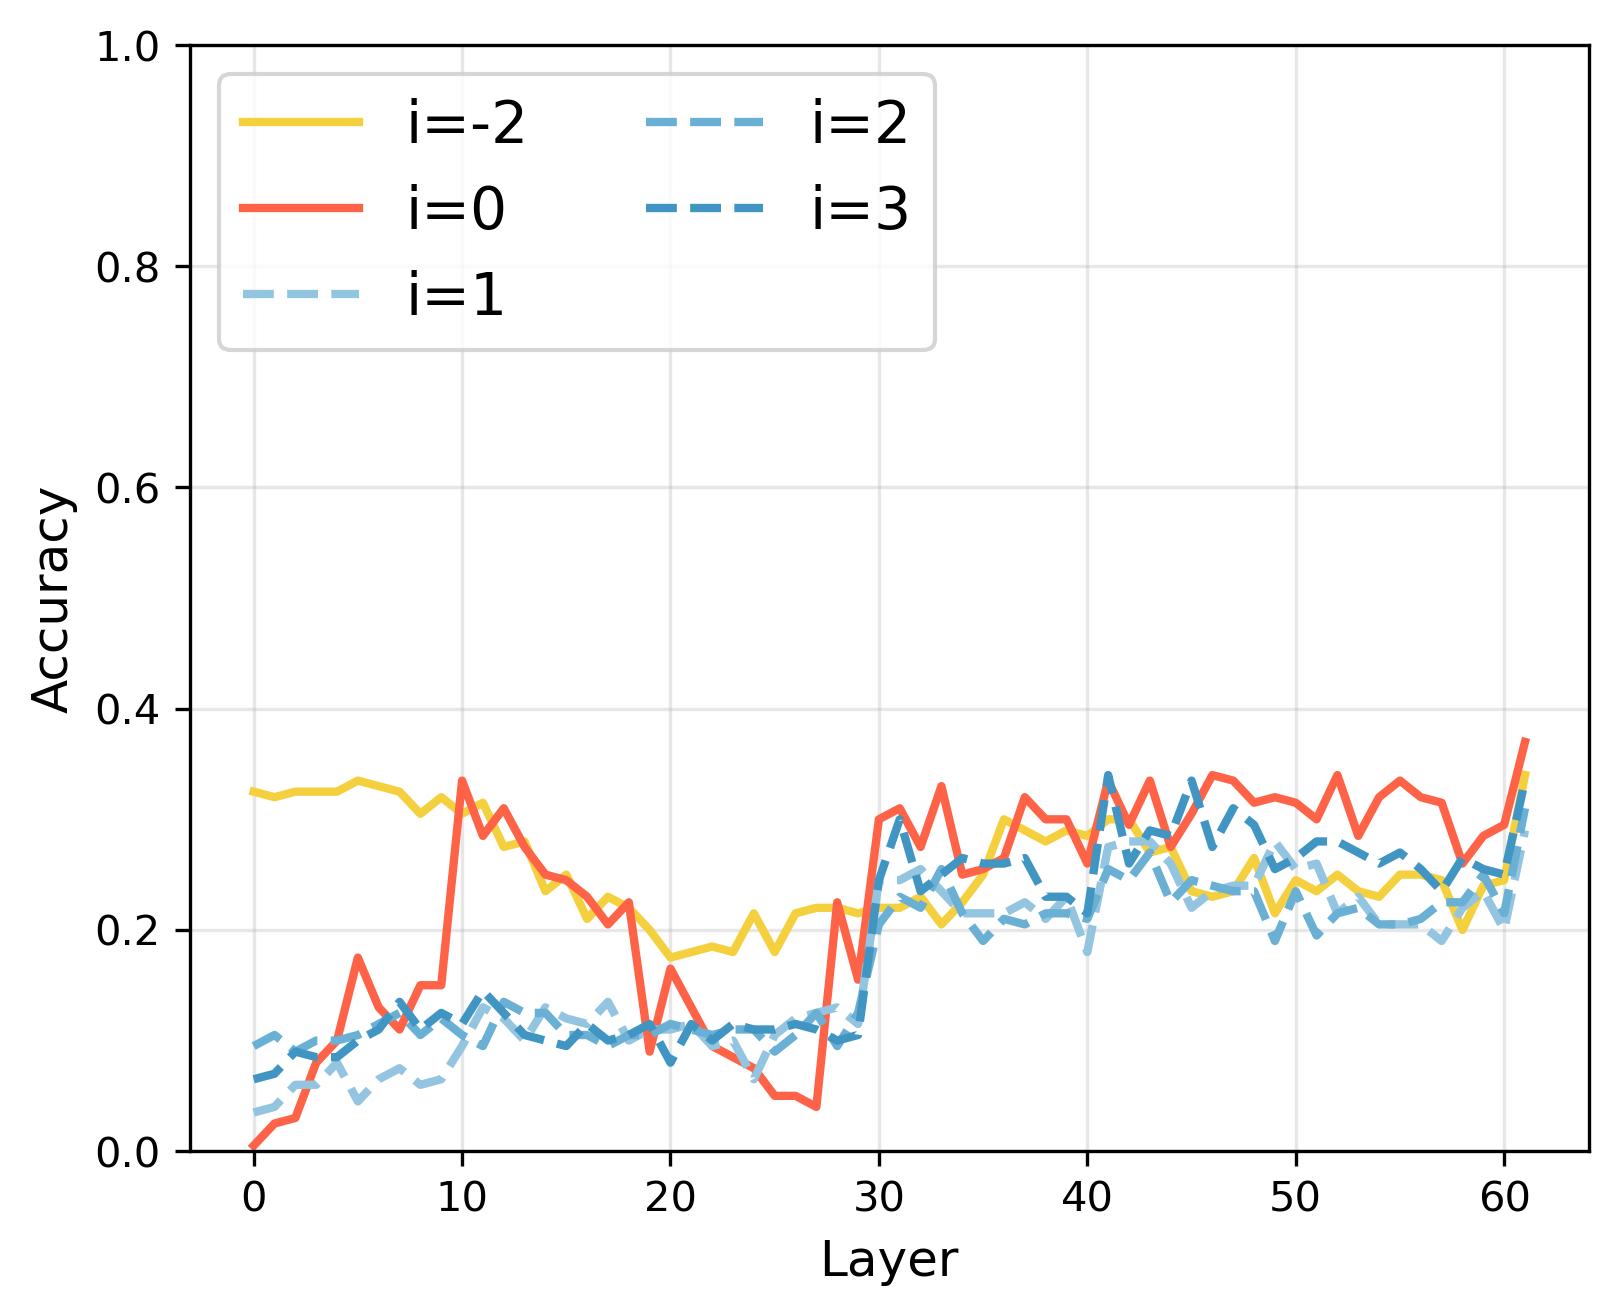
\includegraphics[width=\linewidth]{media/results-poem/gemma-top1.png}
    \end{subfigure}
    \begin{subfigure}{0.49\linewidth}
        \centering
        \subcaption[]{Llama-3.1-8B}
        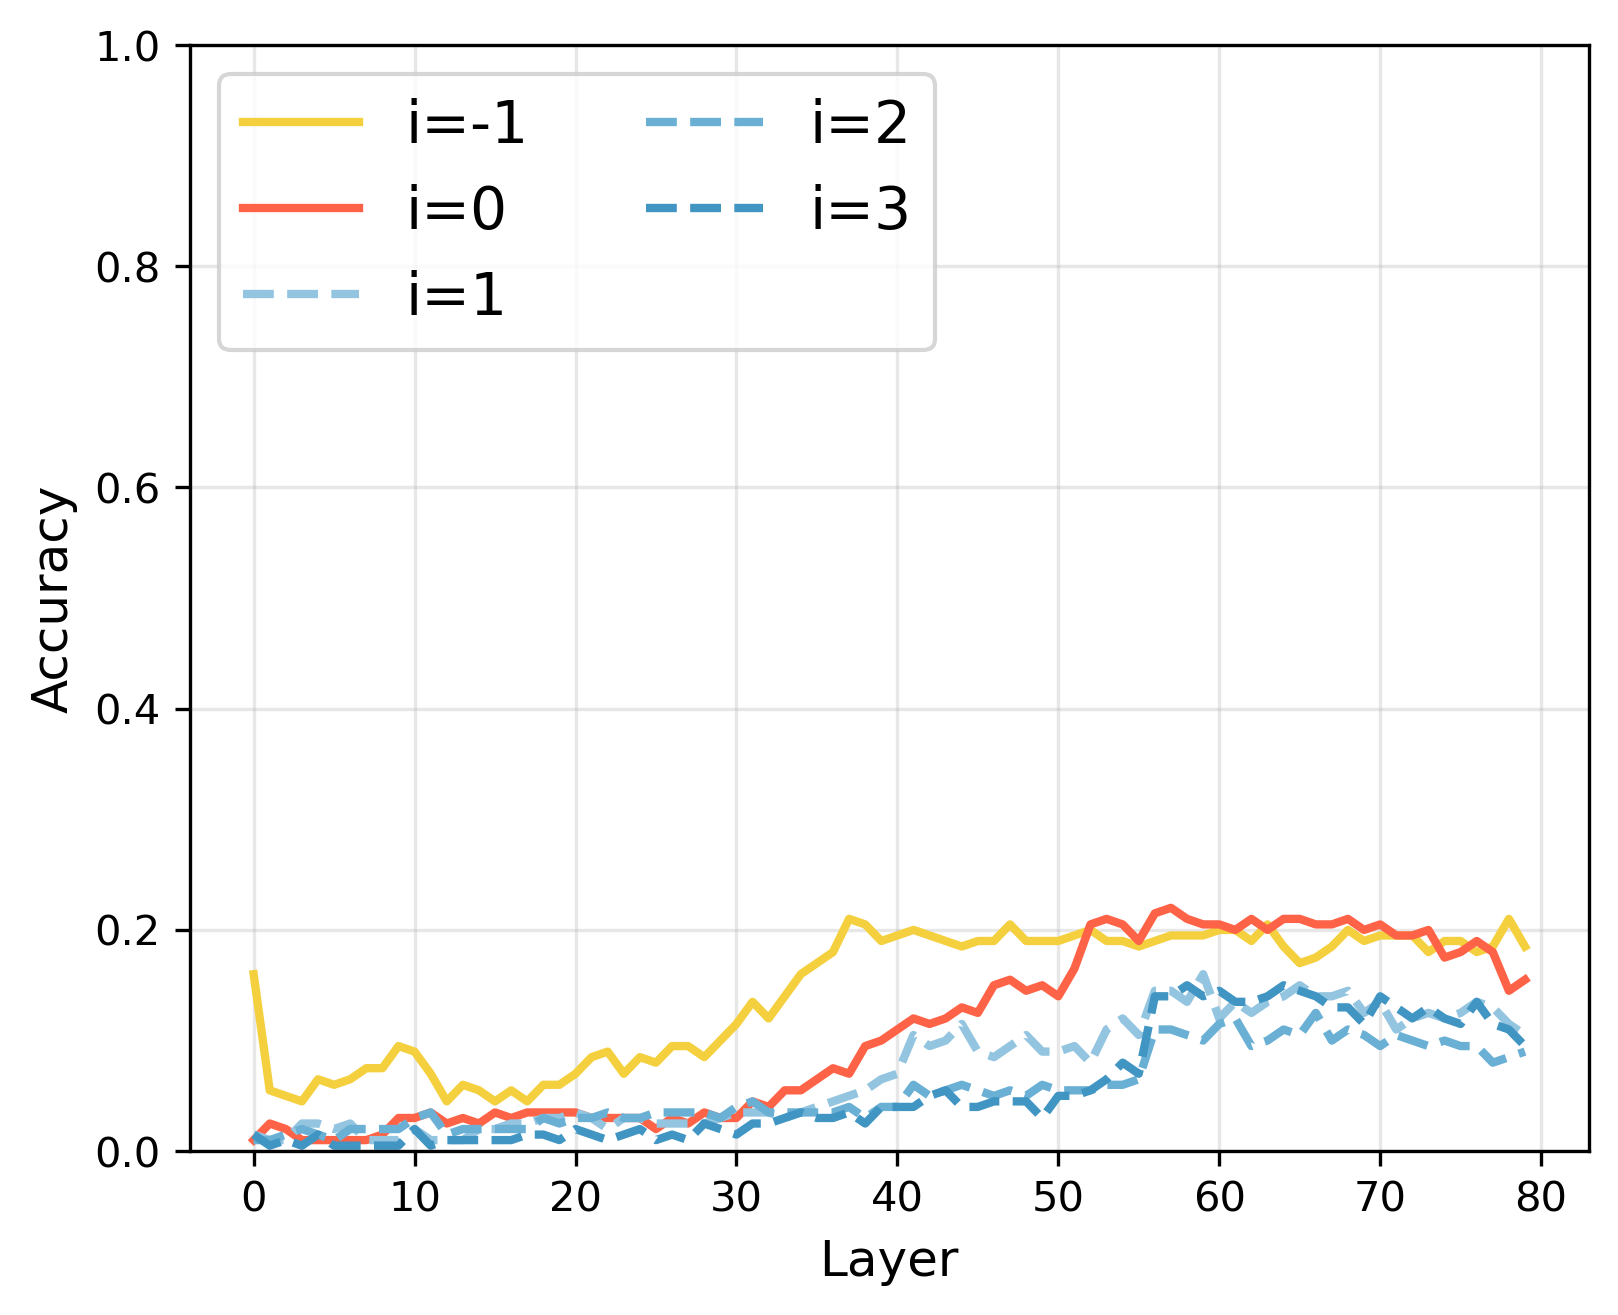
\includegraphics[width=\linewidth]{media/results-poem/llama-top1.png}
    \end{subfigure}
    \caption{Top-1 probe accuracy predicting $r_2$ on rhyming couplets. Mirrors the top-5 and rhyme accuracy results: the $i\leq0$ probes show substantially higher accuracy in middle-to-late layers than probes at $i>0$.}
    \label{fig:appendix-poem}
\end{figure}


\section{Additional Activation Patching Details}
\label{sec:additional-patching-details}

\subsection*{Baselines}
\label{sec:patching-baselines}

To verify that the observed corrupt rhyme rates reflect the specific encoding of the corrupt rhyme word rather than a generic effect of perturbing the residual stream, we run two control conditions. The \textit{zero-vector} baseline replaces the patched hidden state with an all-zeros vector. The \textit{donor-prompt} baseline replaces it with a hidden state cached from the same token position in a semantically unrelated sentence (``The weather outside is warm and sunny today, and the birds are singing.'').

Figure~\ref{fig:patching-baselines} shows results for Qwen3-32B (at $i=-1$) and Gemma-3-27B (at $i=-2$), averaged over all prompt pairs. Both control conditions produce corrupt rhyme rates near zero across all layers, while true activation patching reaches ${\sim}0.80$ for Gemma-3-27B and ${\sim}0.70$ for Qwen3-32B at their peak layers.

\begin{figure}[H]
    \centering
    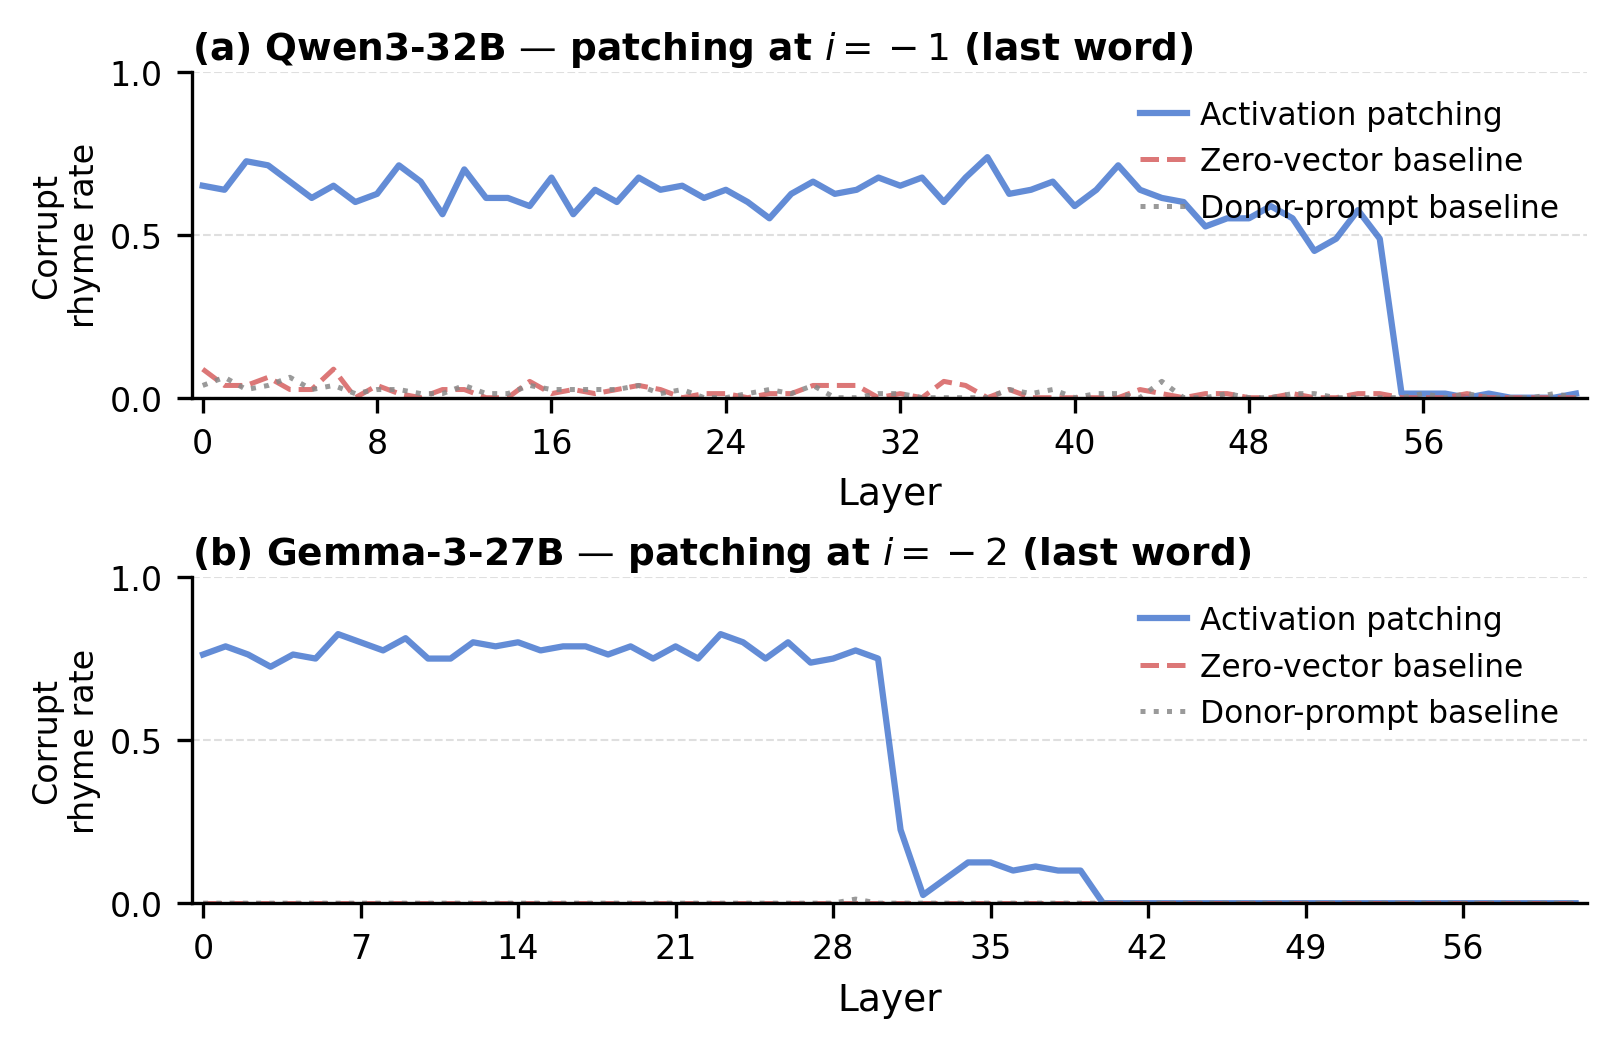
\includegraphics[width=\linewidth]{media/results-patching/patching_baselines.png}
    \caption{Corrupt rhyme rate under true activation patching versus zero-vector and donor-prompt baseline controls at the last word position. Both baselines yield near-zero rates across all layers, confirming that the patching effect is specific to the corrupt rhyme word's identity rather than an artifact of residual stream disruption.}
    \label{fig:patching-baselines}
\end{figure}

\subsection*{All-Layers Patching}
\label{sec:patch-all-layers}

Table~\ref{tab:patch-all-layers} reports corrupt rhyme rates when all layers are patched simultaneously at a given token position. Positions $i \geq 1$ yield zero corrupt rhyme rate in every model and are omitted.

\begin{table}[h]
\centering
\begin{tabular}{llcc}
\toprule
Family & Model & Last Word & $i=0$ \\
\midrule
\multirow{6}{*}{Qwen3}
 & 0.6B  &  1 &  7 \\
 & 1.7B  & 15 &  2 \\
 & 4B    & 42 &  7 \\
 & 8B    & 53 &  2 \\
 & 14B   & 63 &  7 \\
 & 32B   & 96 &  9 \\
\midrule
\multirow{4}{*}{Gemma-3}
 & 1B    & 37 &  1 \\
 & 4B    & 78 &  0 \\
 & 12B   & 90 &  0 \\
 & 27B   & 100 & 73 \\
\midrule
\multirow{3}{*}{Llama-3}
 & 1B    & 59 &  2 \\
 & 3B    & 87 &  0 \\
 & 8B    & 79 &  0 \\
\bottomrule
\end{tabular}
\caption{Corrupt rhyme rate (\%) when all layers are patched simultaneously. Gemma-3-27B is the only model with substantial newline effectiveness.}
\label{tab:patch-all-layers}
\end{table}

\subsection*{Per-Layer Results: All Models}

\begin{figure}[H]
    \centering
    
\includegraphics[width=\linewidth]{media/results-patching/patching_summary_bars.png}
    \caption{Peak corrupt rhyme rate (maximum across all layers) for the last word token and newline ($i=0$) at each model size. Gemma-3-27B is the only model for which newline patching reaches a substantial level; all Qwen3 and Llama-3 models show near-zero newline effectiveness regardless of scale.}
    \label{fig:appendix-patch-summary}
\end{figure}

\begin{figure}[H]
    \centering
    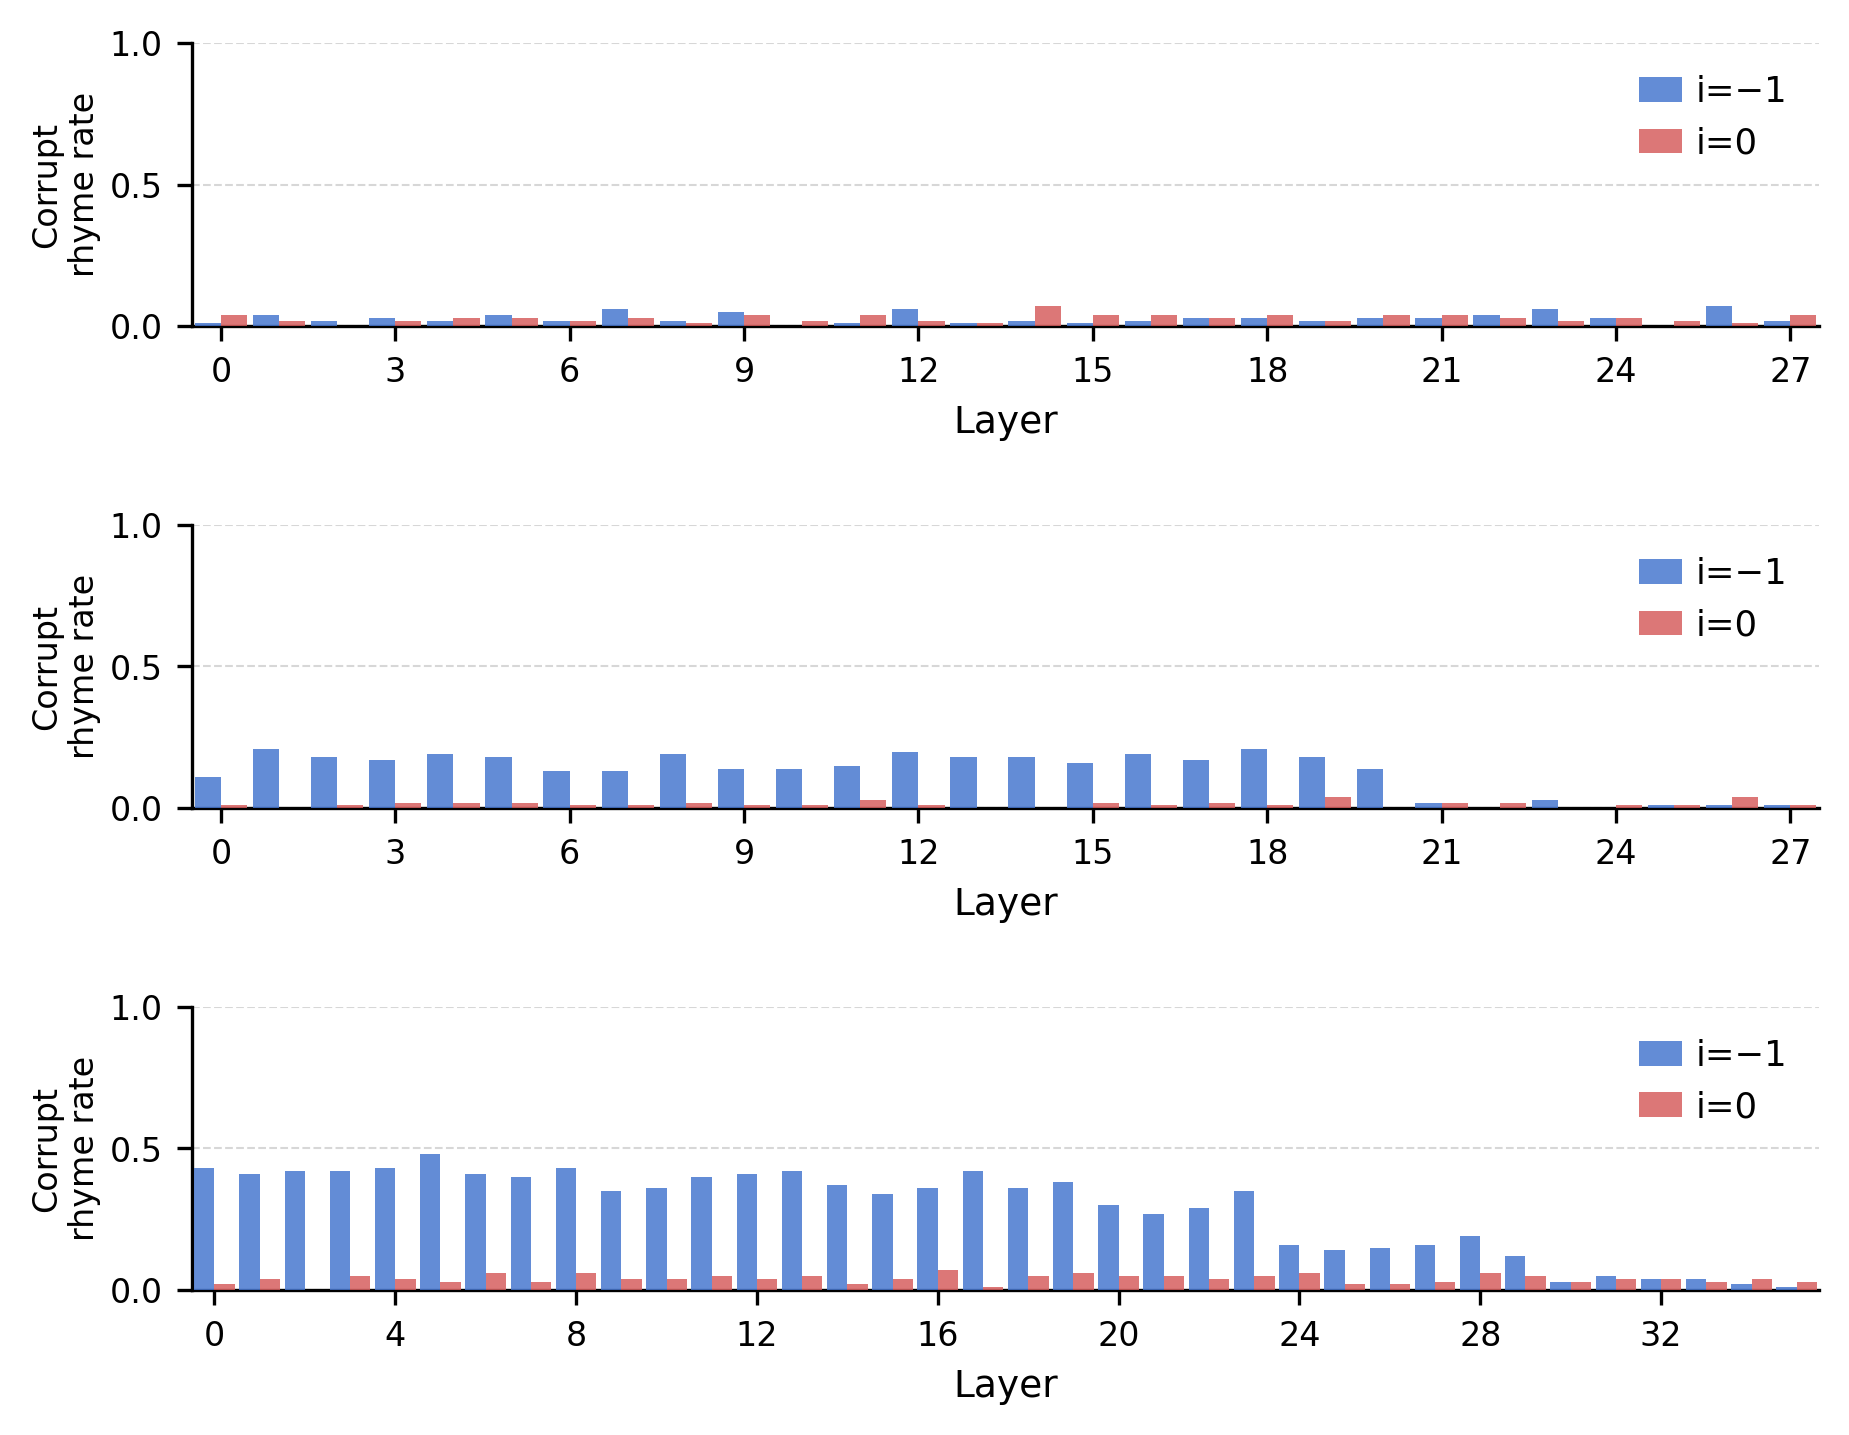
\includegraphics[width=\linewidth]{media/results-patching/appendix_patching_Qwen3_small.png}
    \caption{Per-layer activation patching, Qwen3 0.6B--4B.}
    \label{fig:appendix-patch-qwen3-small}
\end{figure}

\begin{figure}[H]
    \centering
    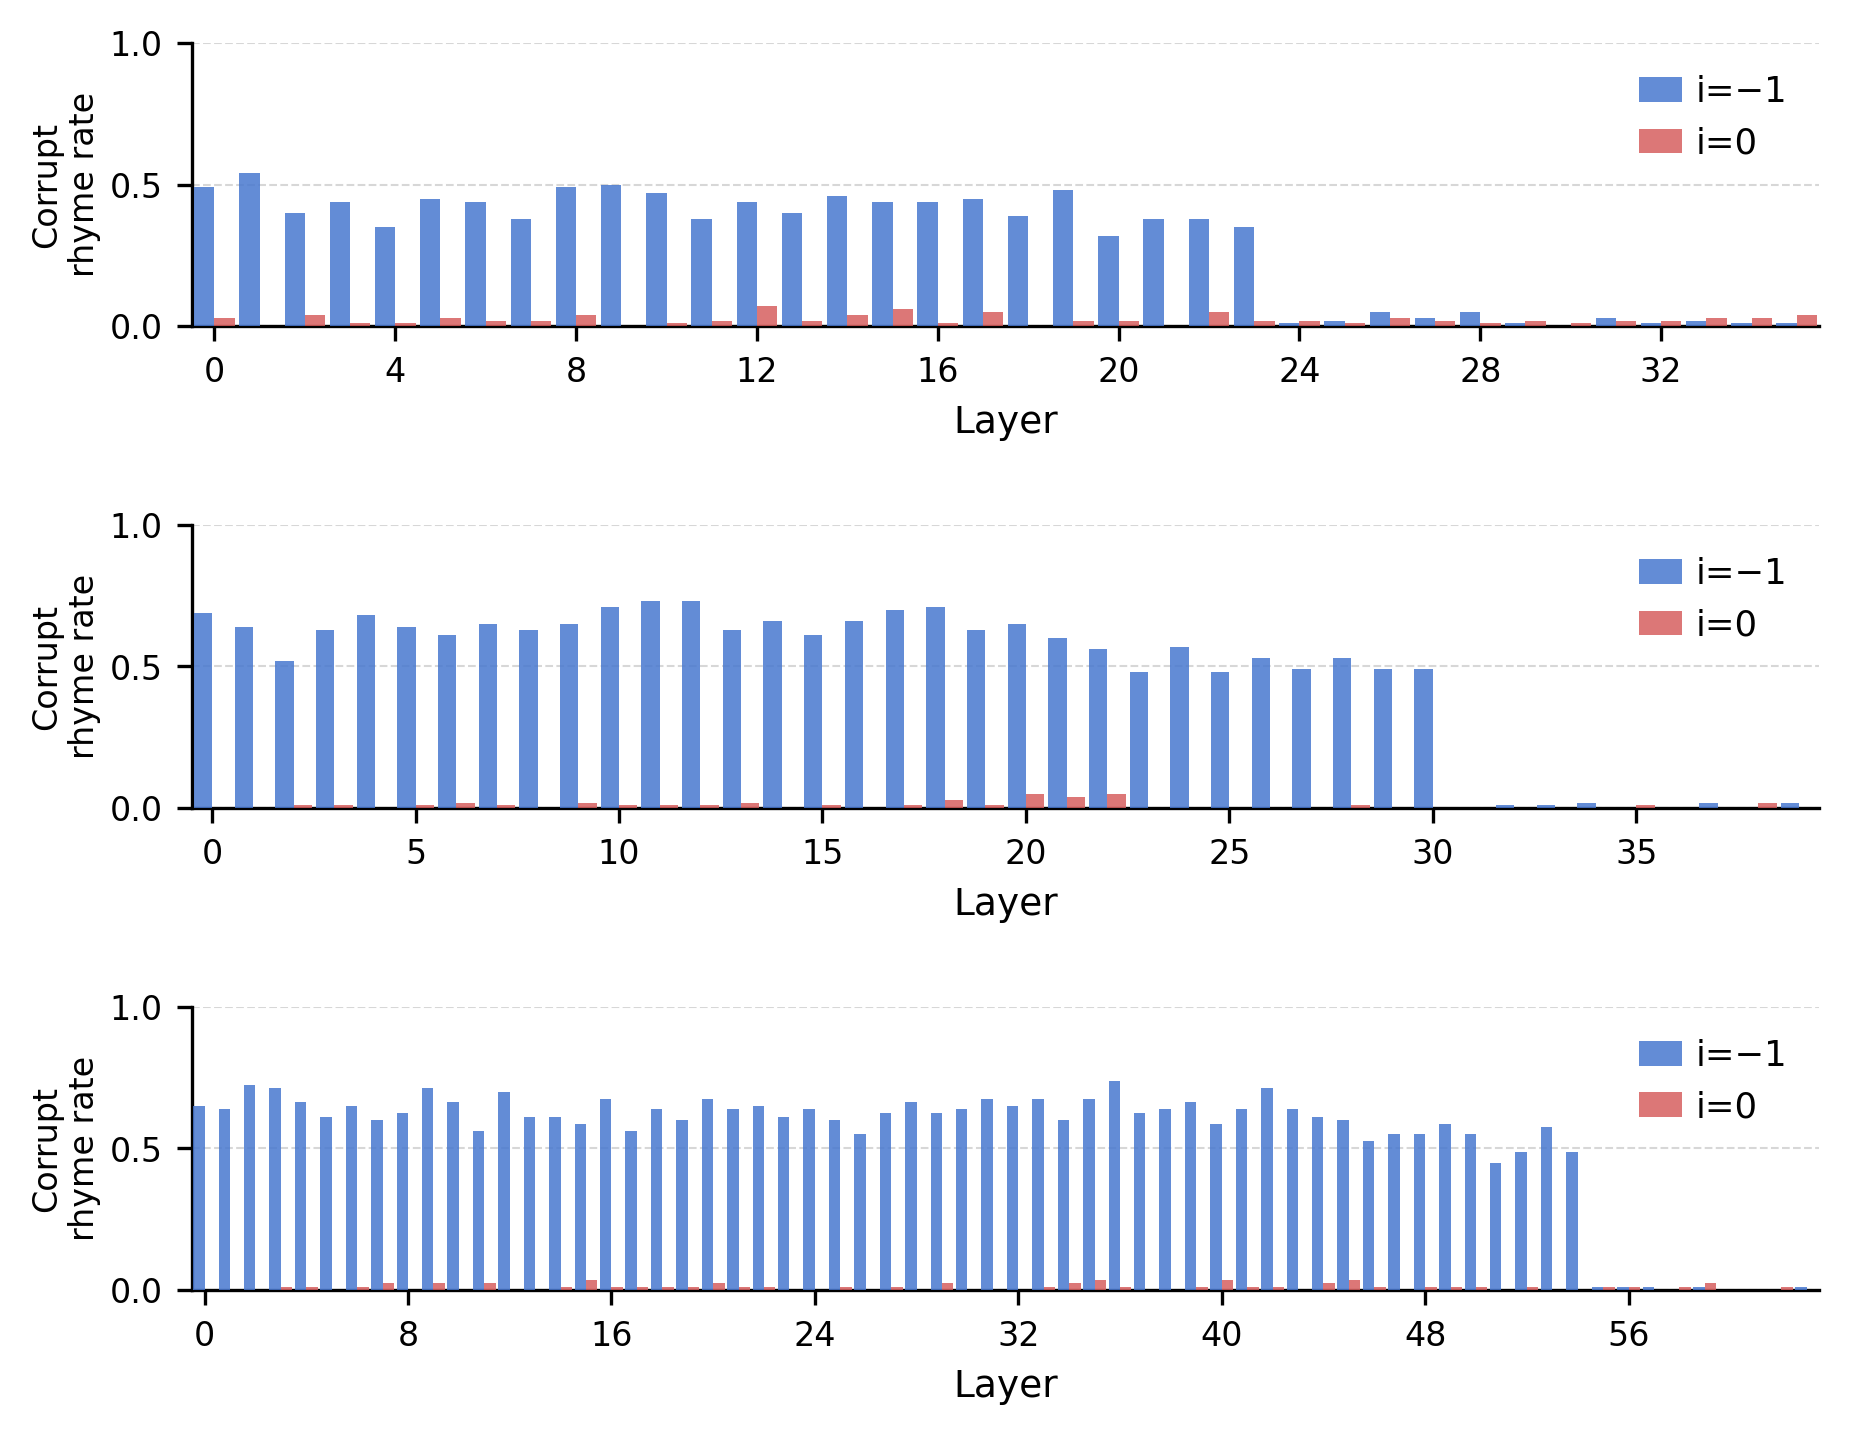
\includegraphics[width=\linewidth]{media/results-patching/appendix_patching_Qwen3_large.png}
    \caption{Per-layer activation patching, Qwen3 8B--32B.}
    \label{fig:appendix-patch-qwen3-large}
\end{figure}

\begin{figure}[H]
    \centering
    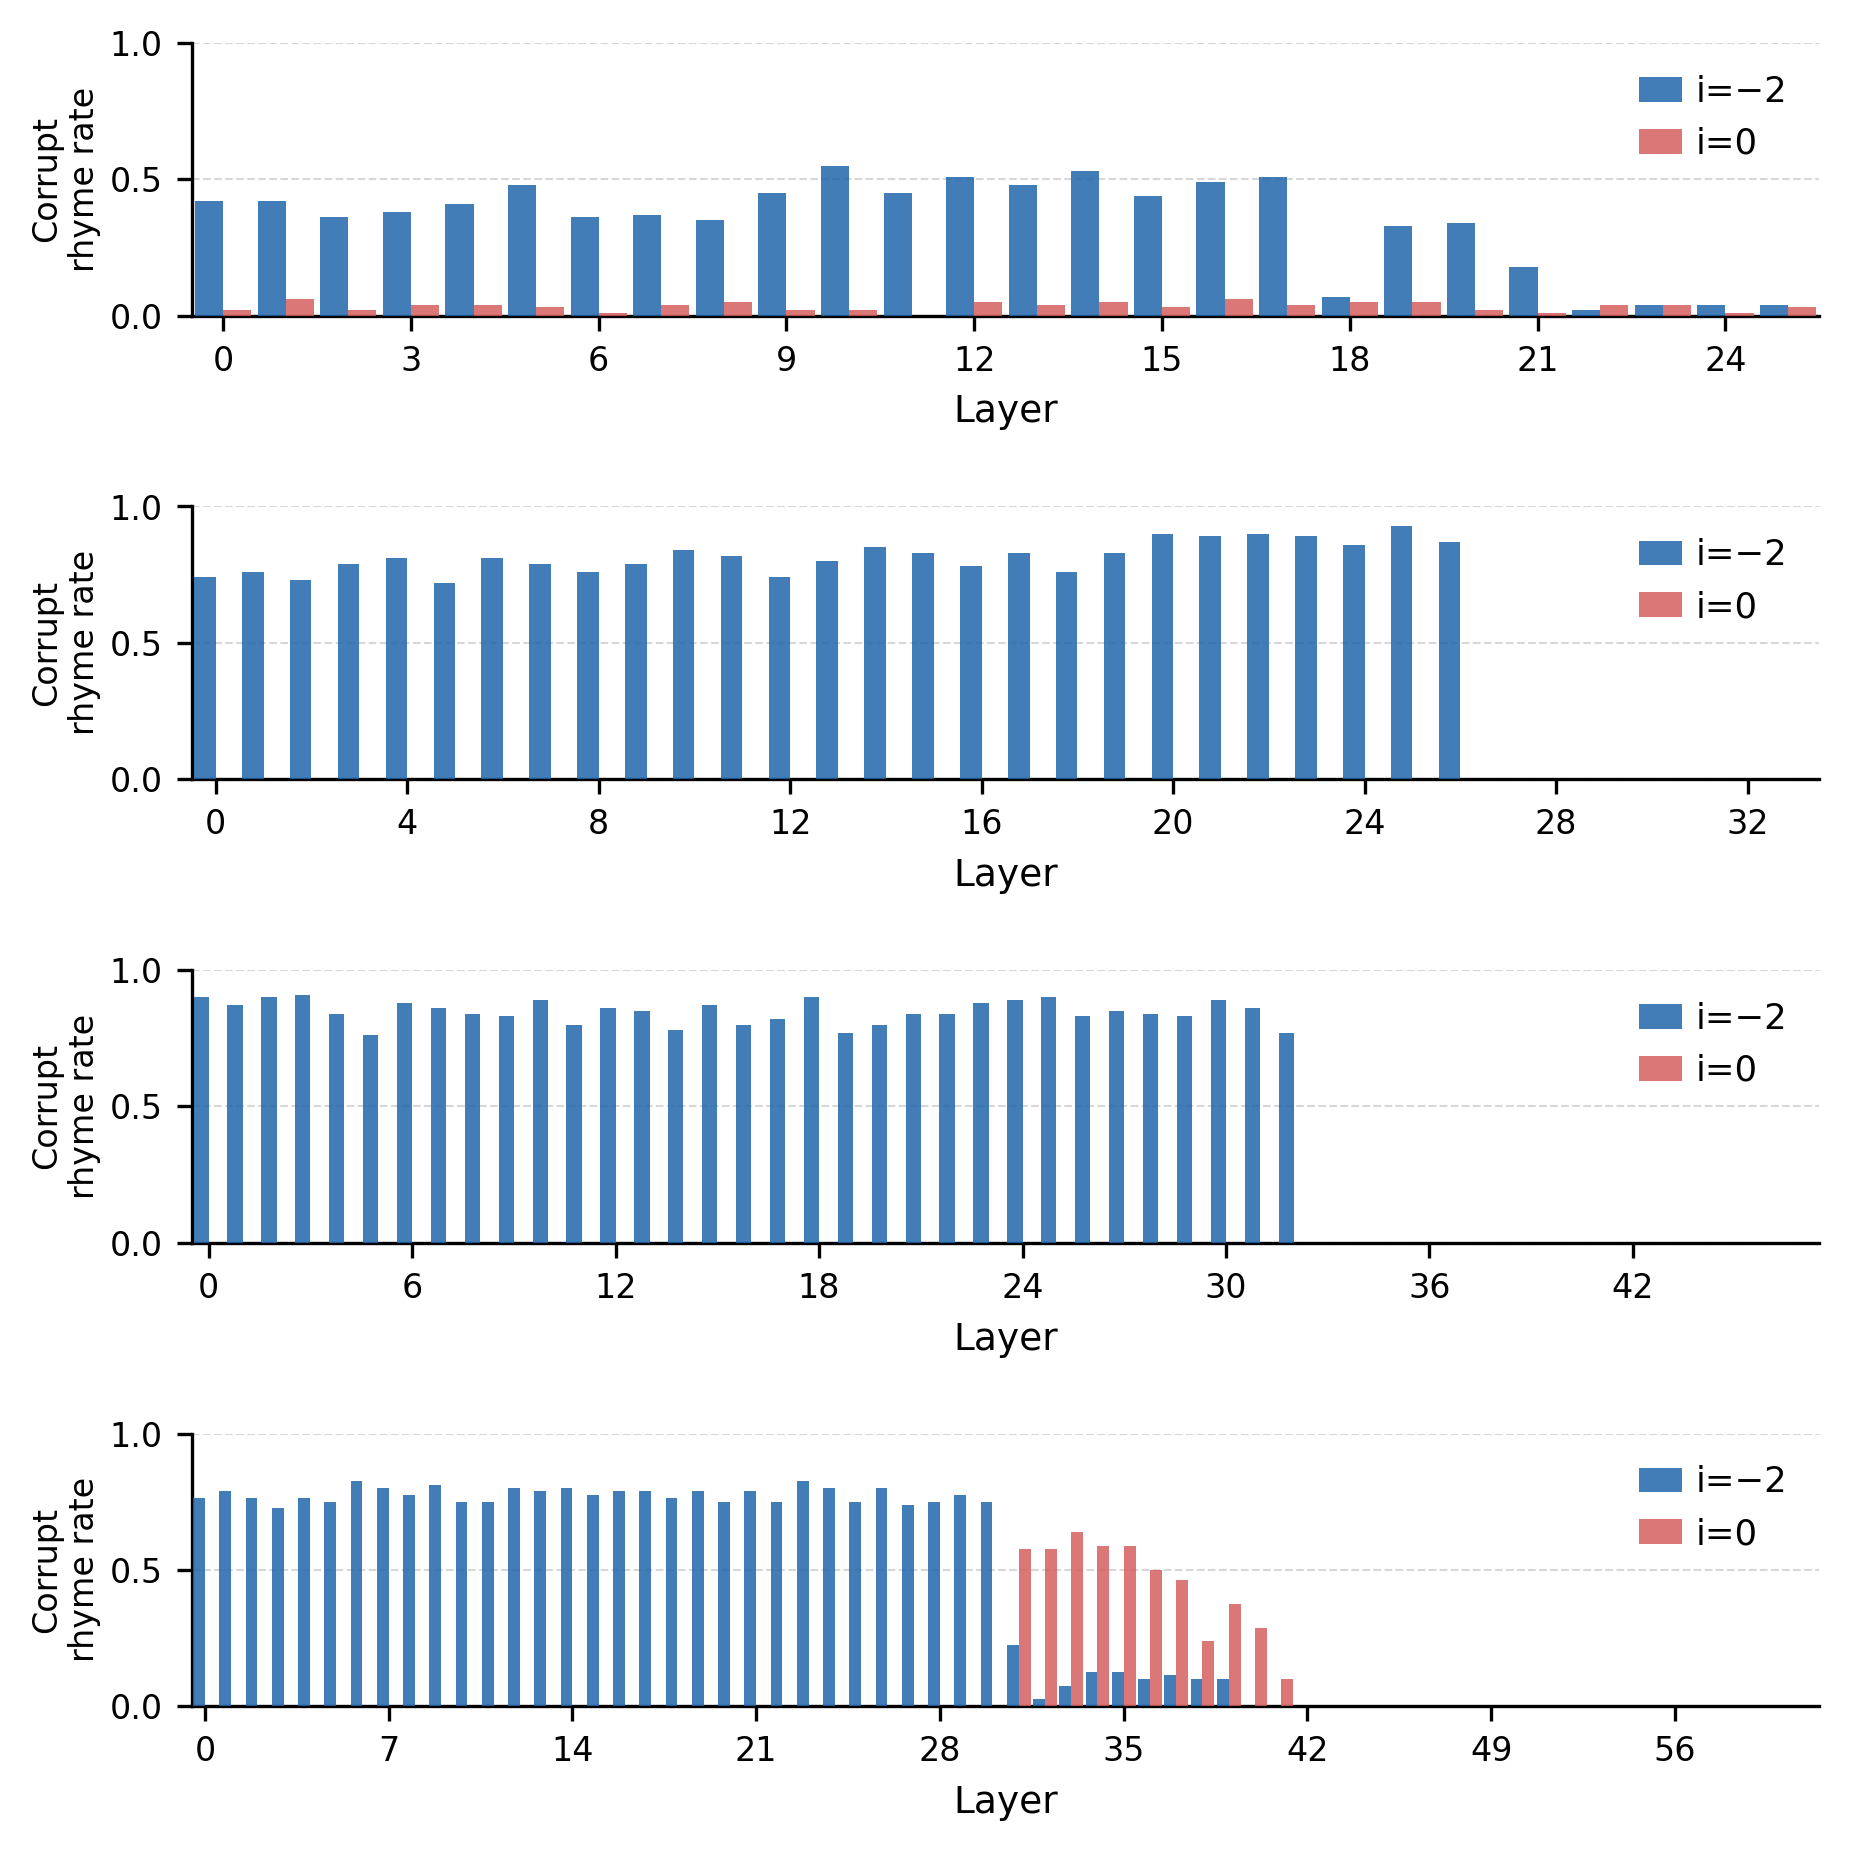
\includegraphics[width=\linewidth]{media/results-patching/appendix_patching_Gemma3.png}
    \caption{Per-layer activation patching, Gemma-3 1B--27B.}
    \label{fig:appendix-patch-gemma3}
\end{figure}

\begin{figure}[H]
    \centering
    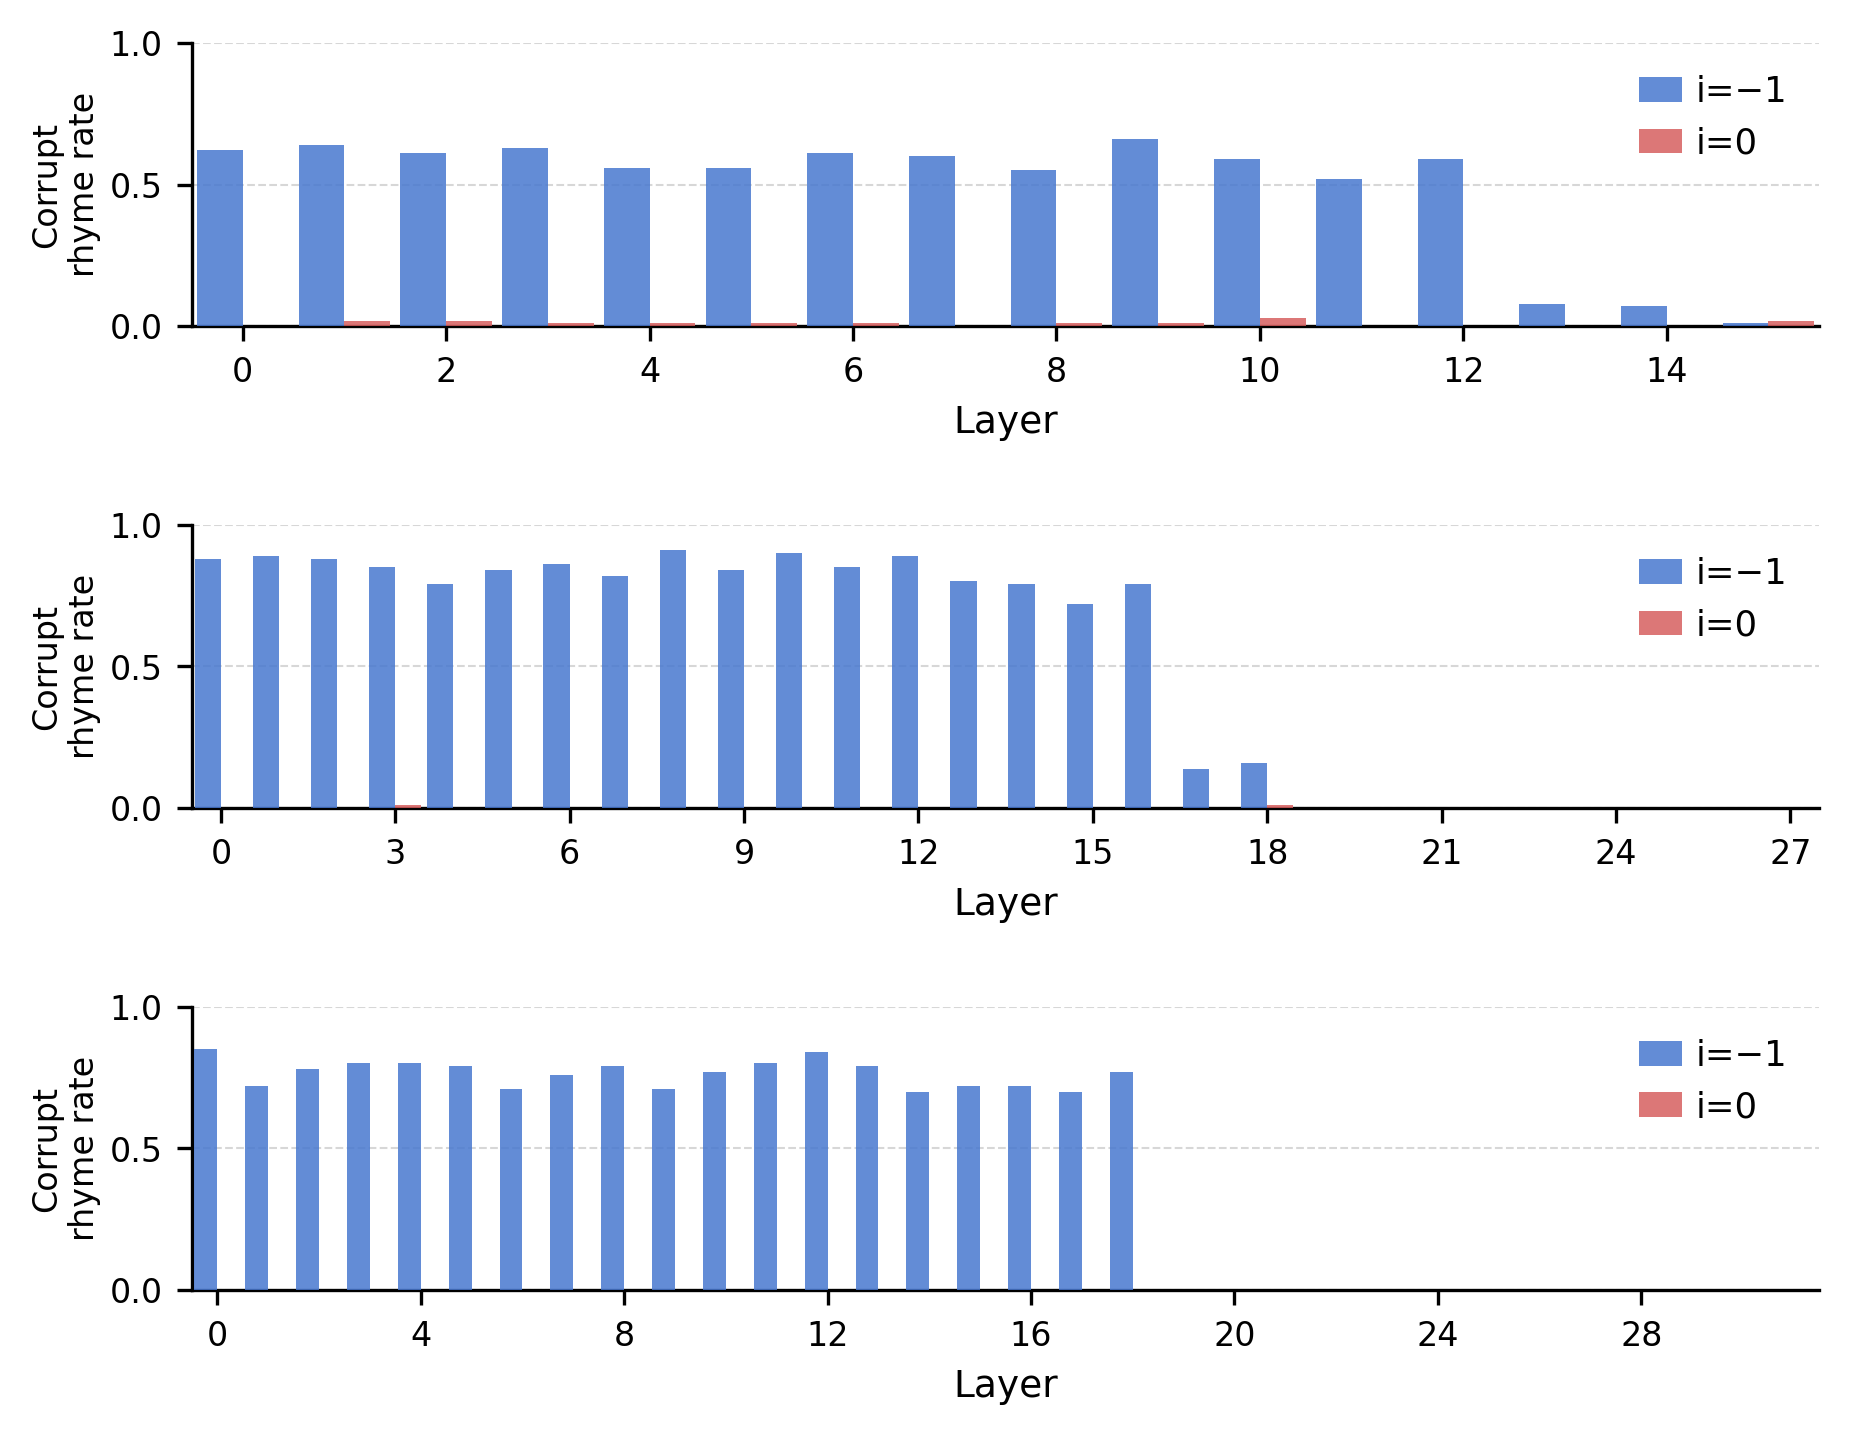
\includegraphics[width=\linewidth]{media/results-patching/appendix_patching_Llama3.png}
    \caption{Per-layer activation patching, Llama-3 1B--8B.}
    \label{fig:appendix-patch-llama3}
\end{figure}

\subsection*{Full Position Sweep}
\label{sec:additional-patching-sweep}

\begin{figure}[H]
    \centering
    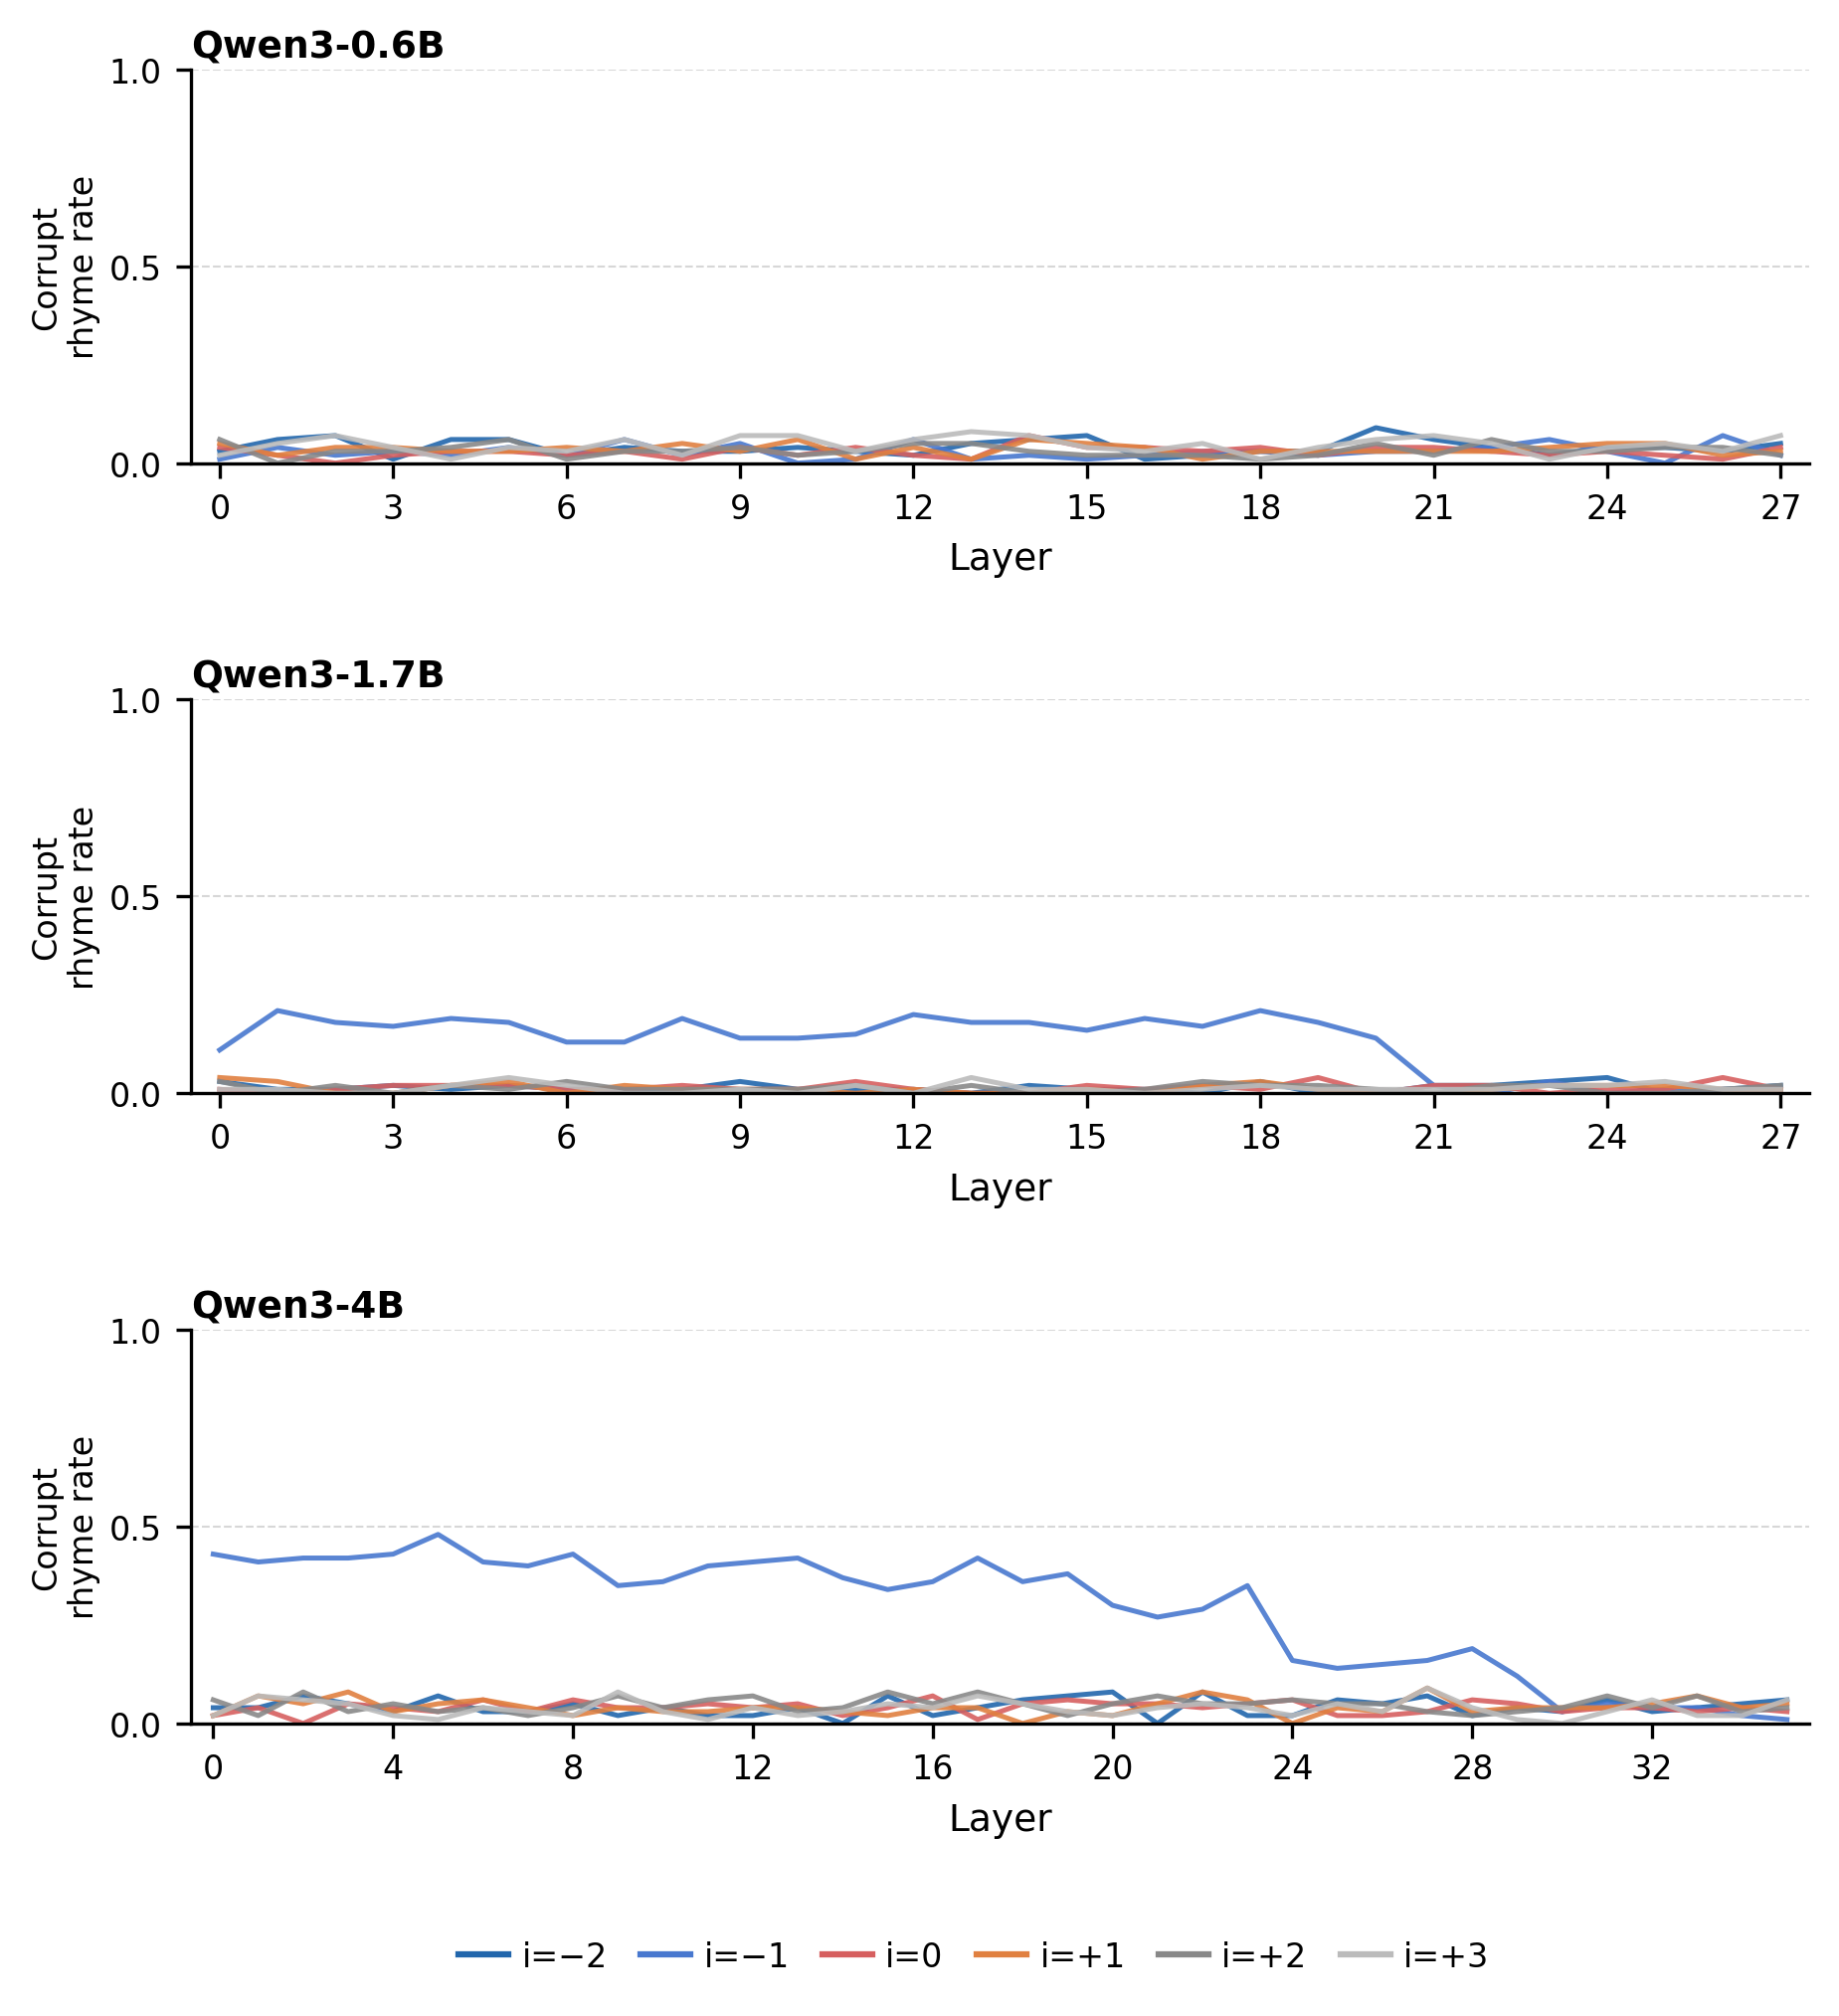
\includegraphics[width=\linewidth]{media/results-patching/appendix_sweep_Qwen3_small.png}
    \caption{Full position sweep, Qwen3 0.6B--4B.}
    \label{fig:appendix-sweep-qwen3-small}
\end{figure}

\begin{figure}[H]
    \centering
    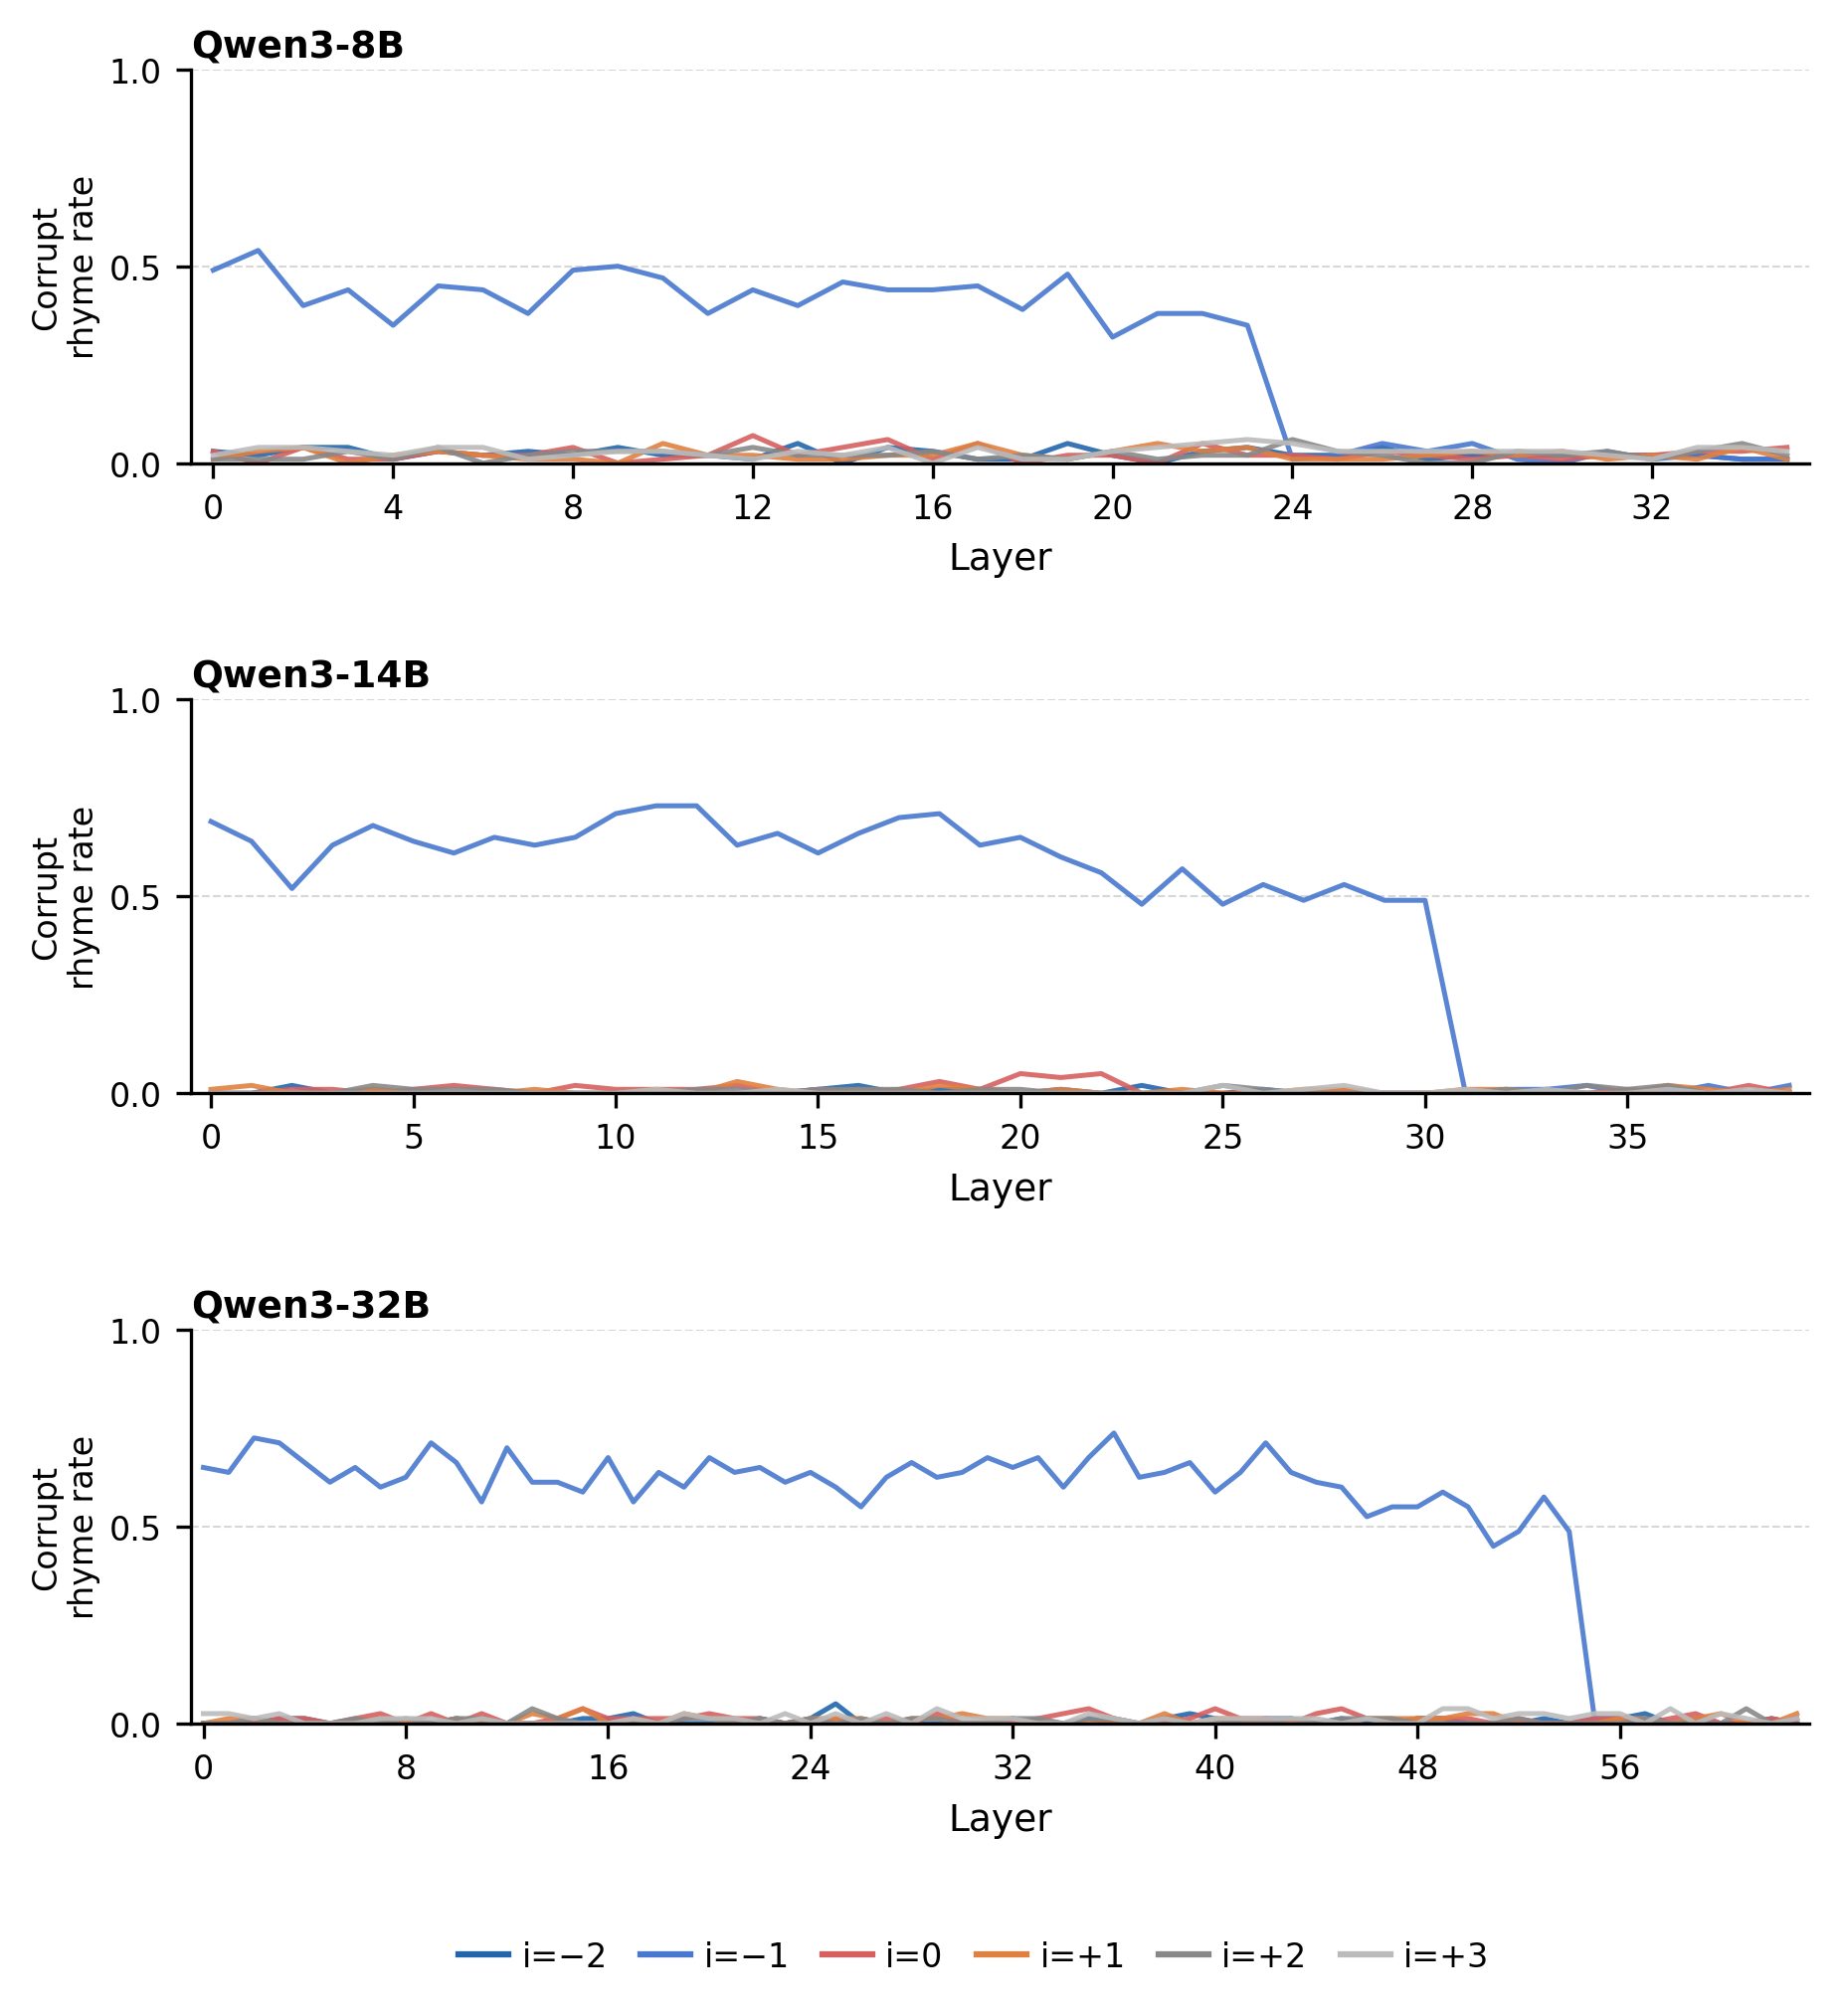
\includegraphics[width=\linewidth]{media/results-patching/appendix_sweep_Qwen3_large.png}
    \caption{Full position sweep, Qwen3 8B--32B.}
    \label{fig:appendix-sweep-qwen3-large}
\end{figure}

\begin{figure}[H]
    \centering
    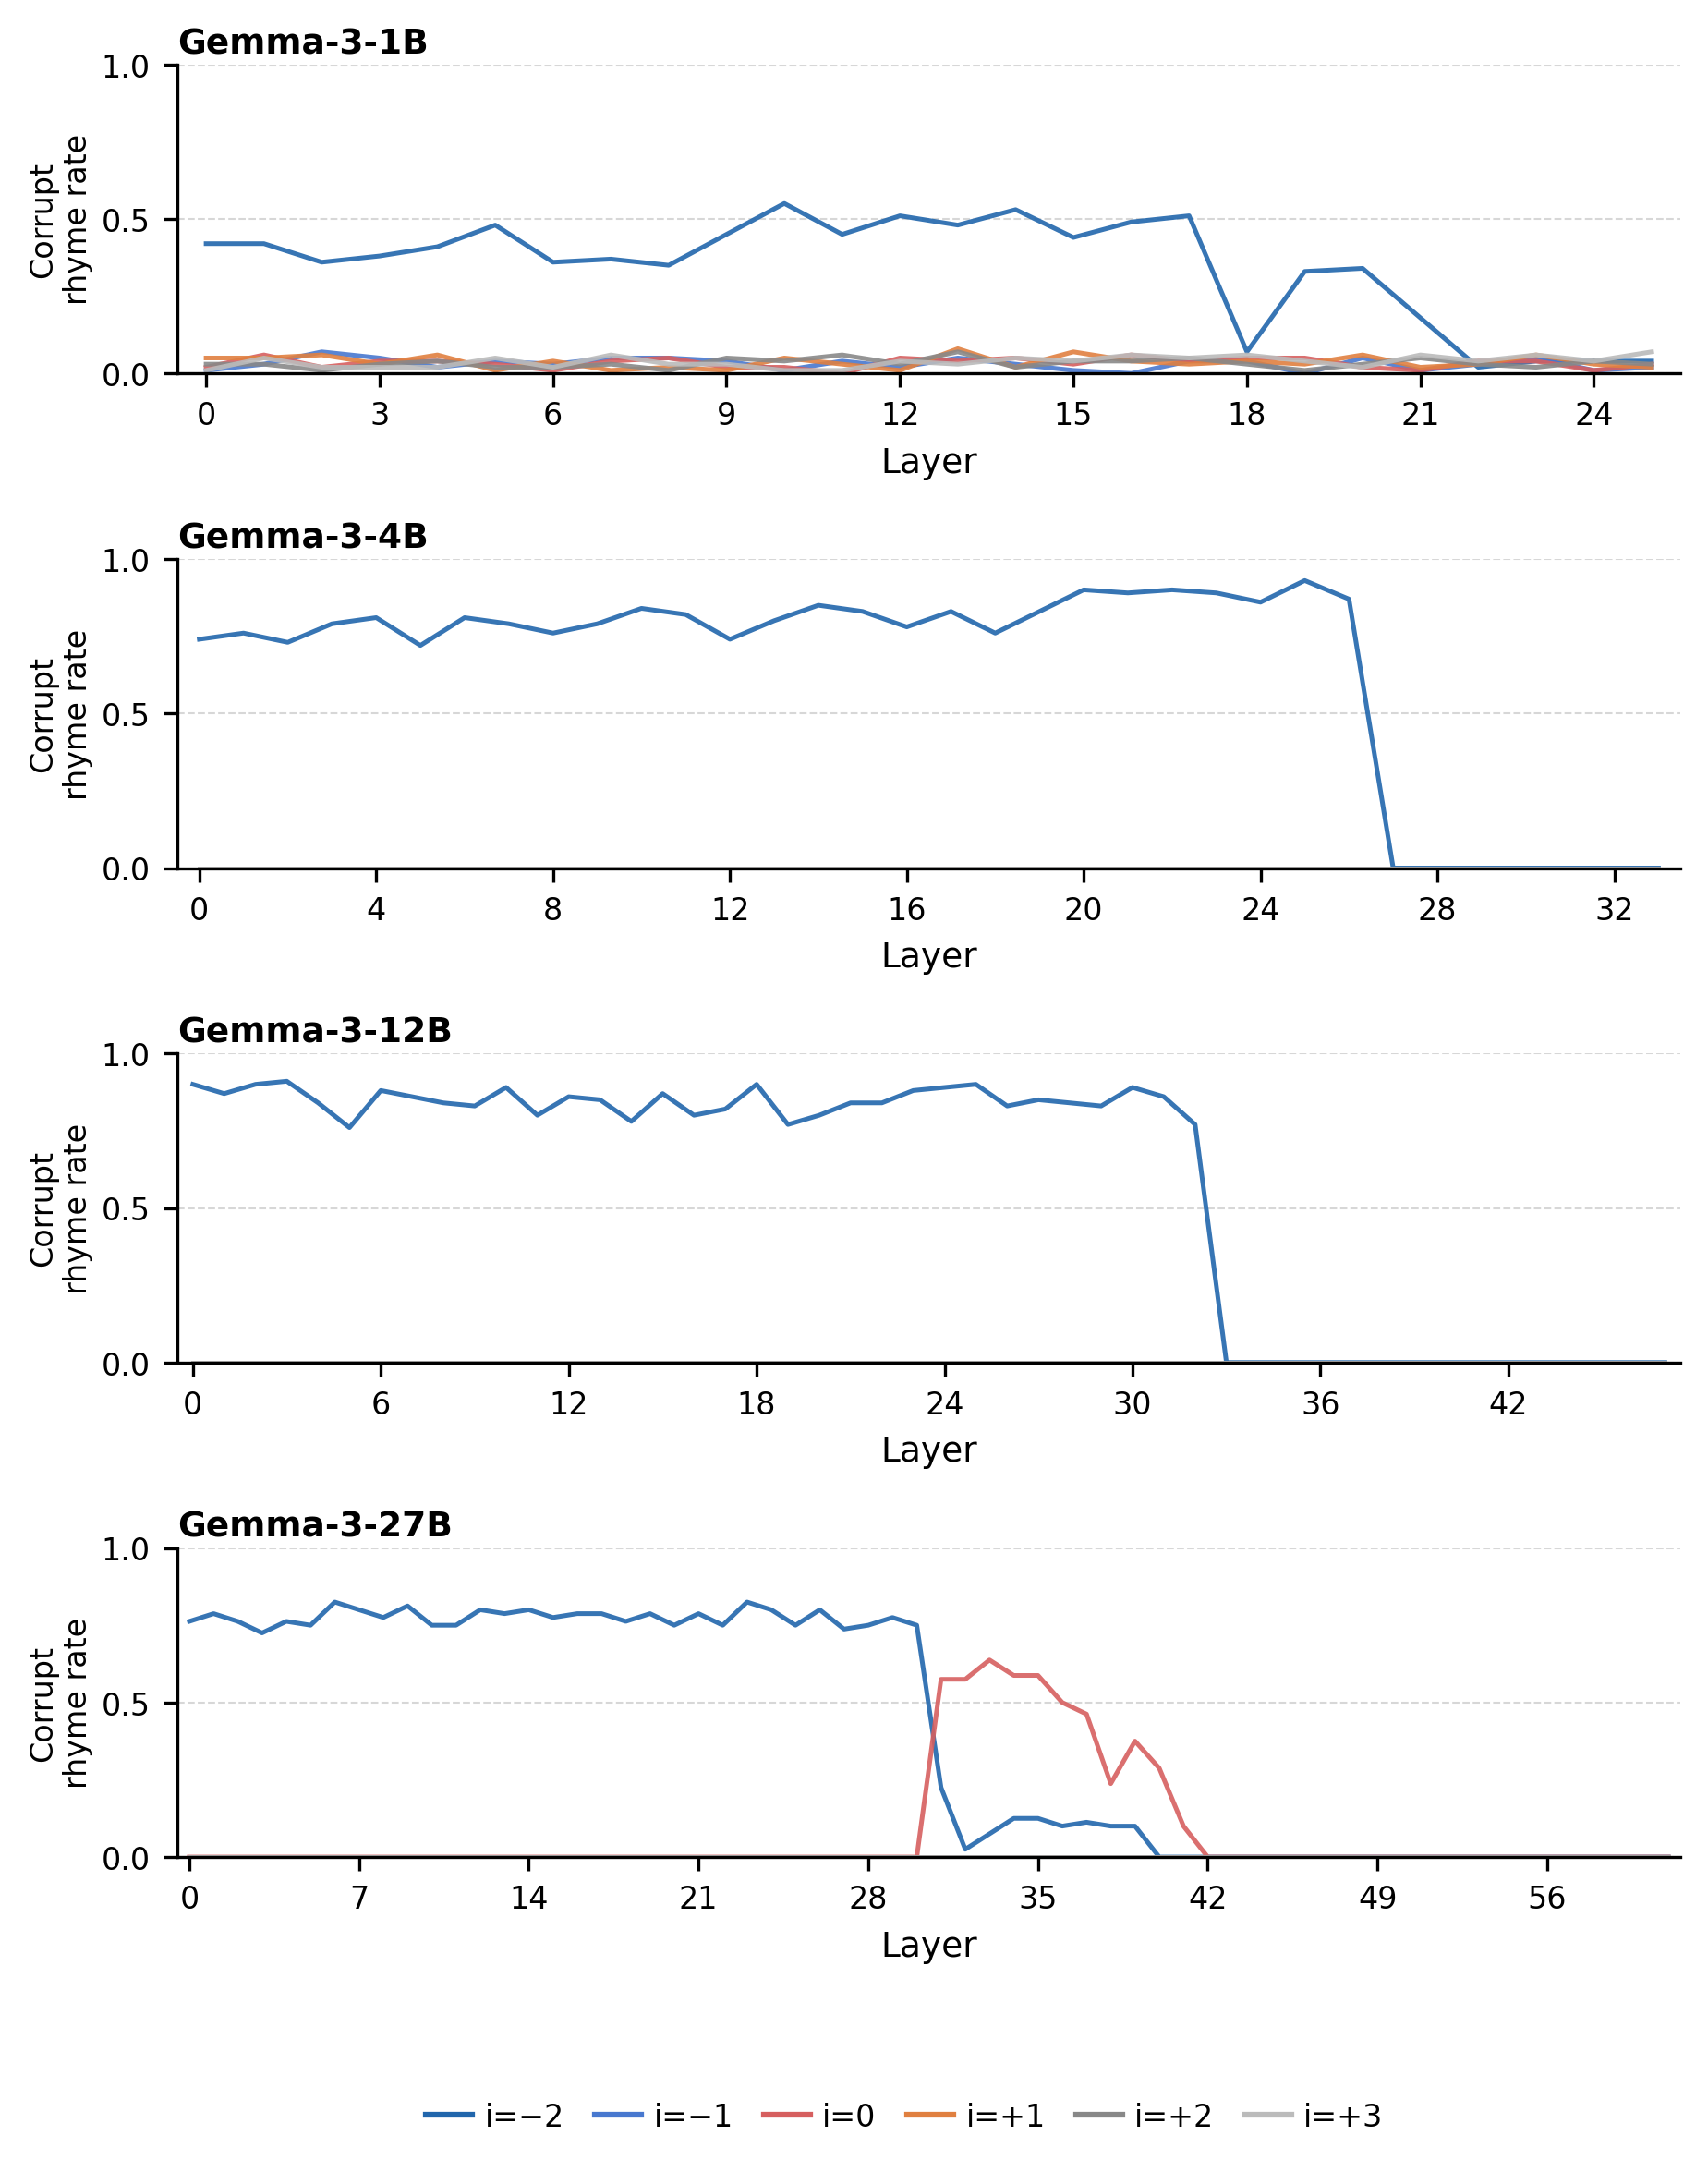
\includegraphics[width=\linewidth]{media/results-patching/appendix_sweep_Gemma3.png}
    \caption{Full position sweep, Gemma-3 1B--27B.}
    \label{fig:appendix-sweep-gemma3}
\end{figure}

\begin{figure}[H]
    \centering
    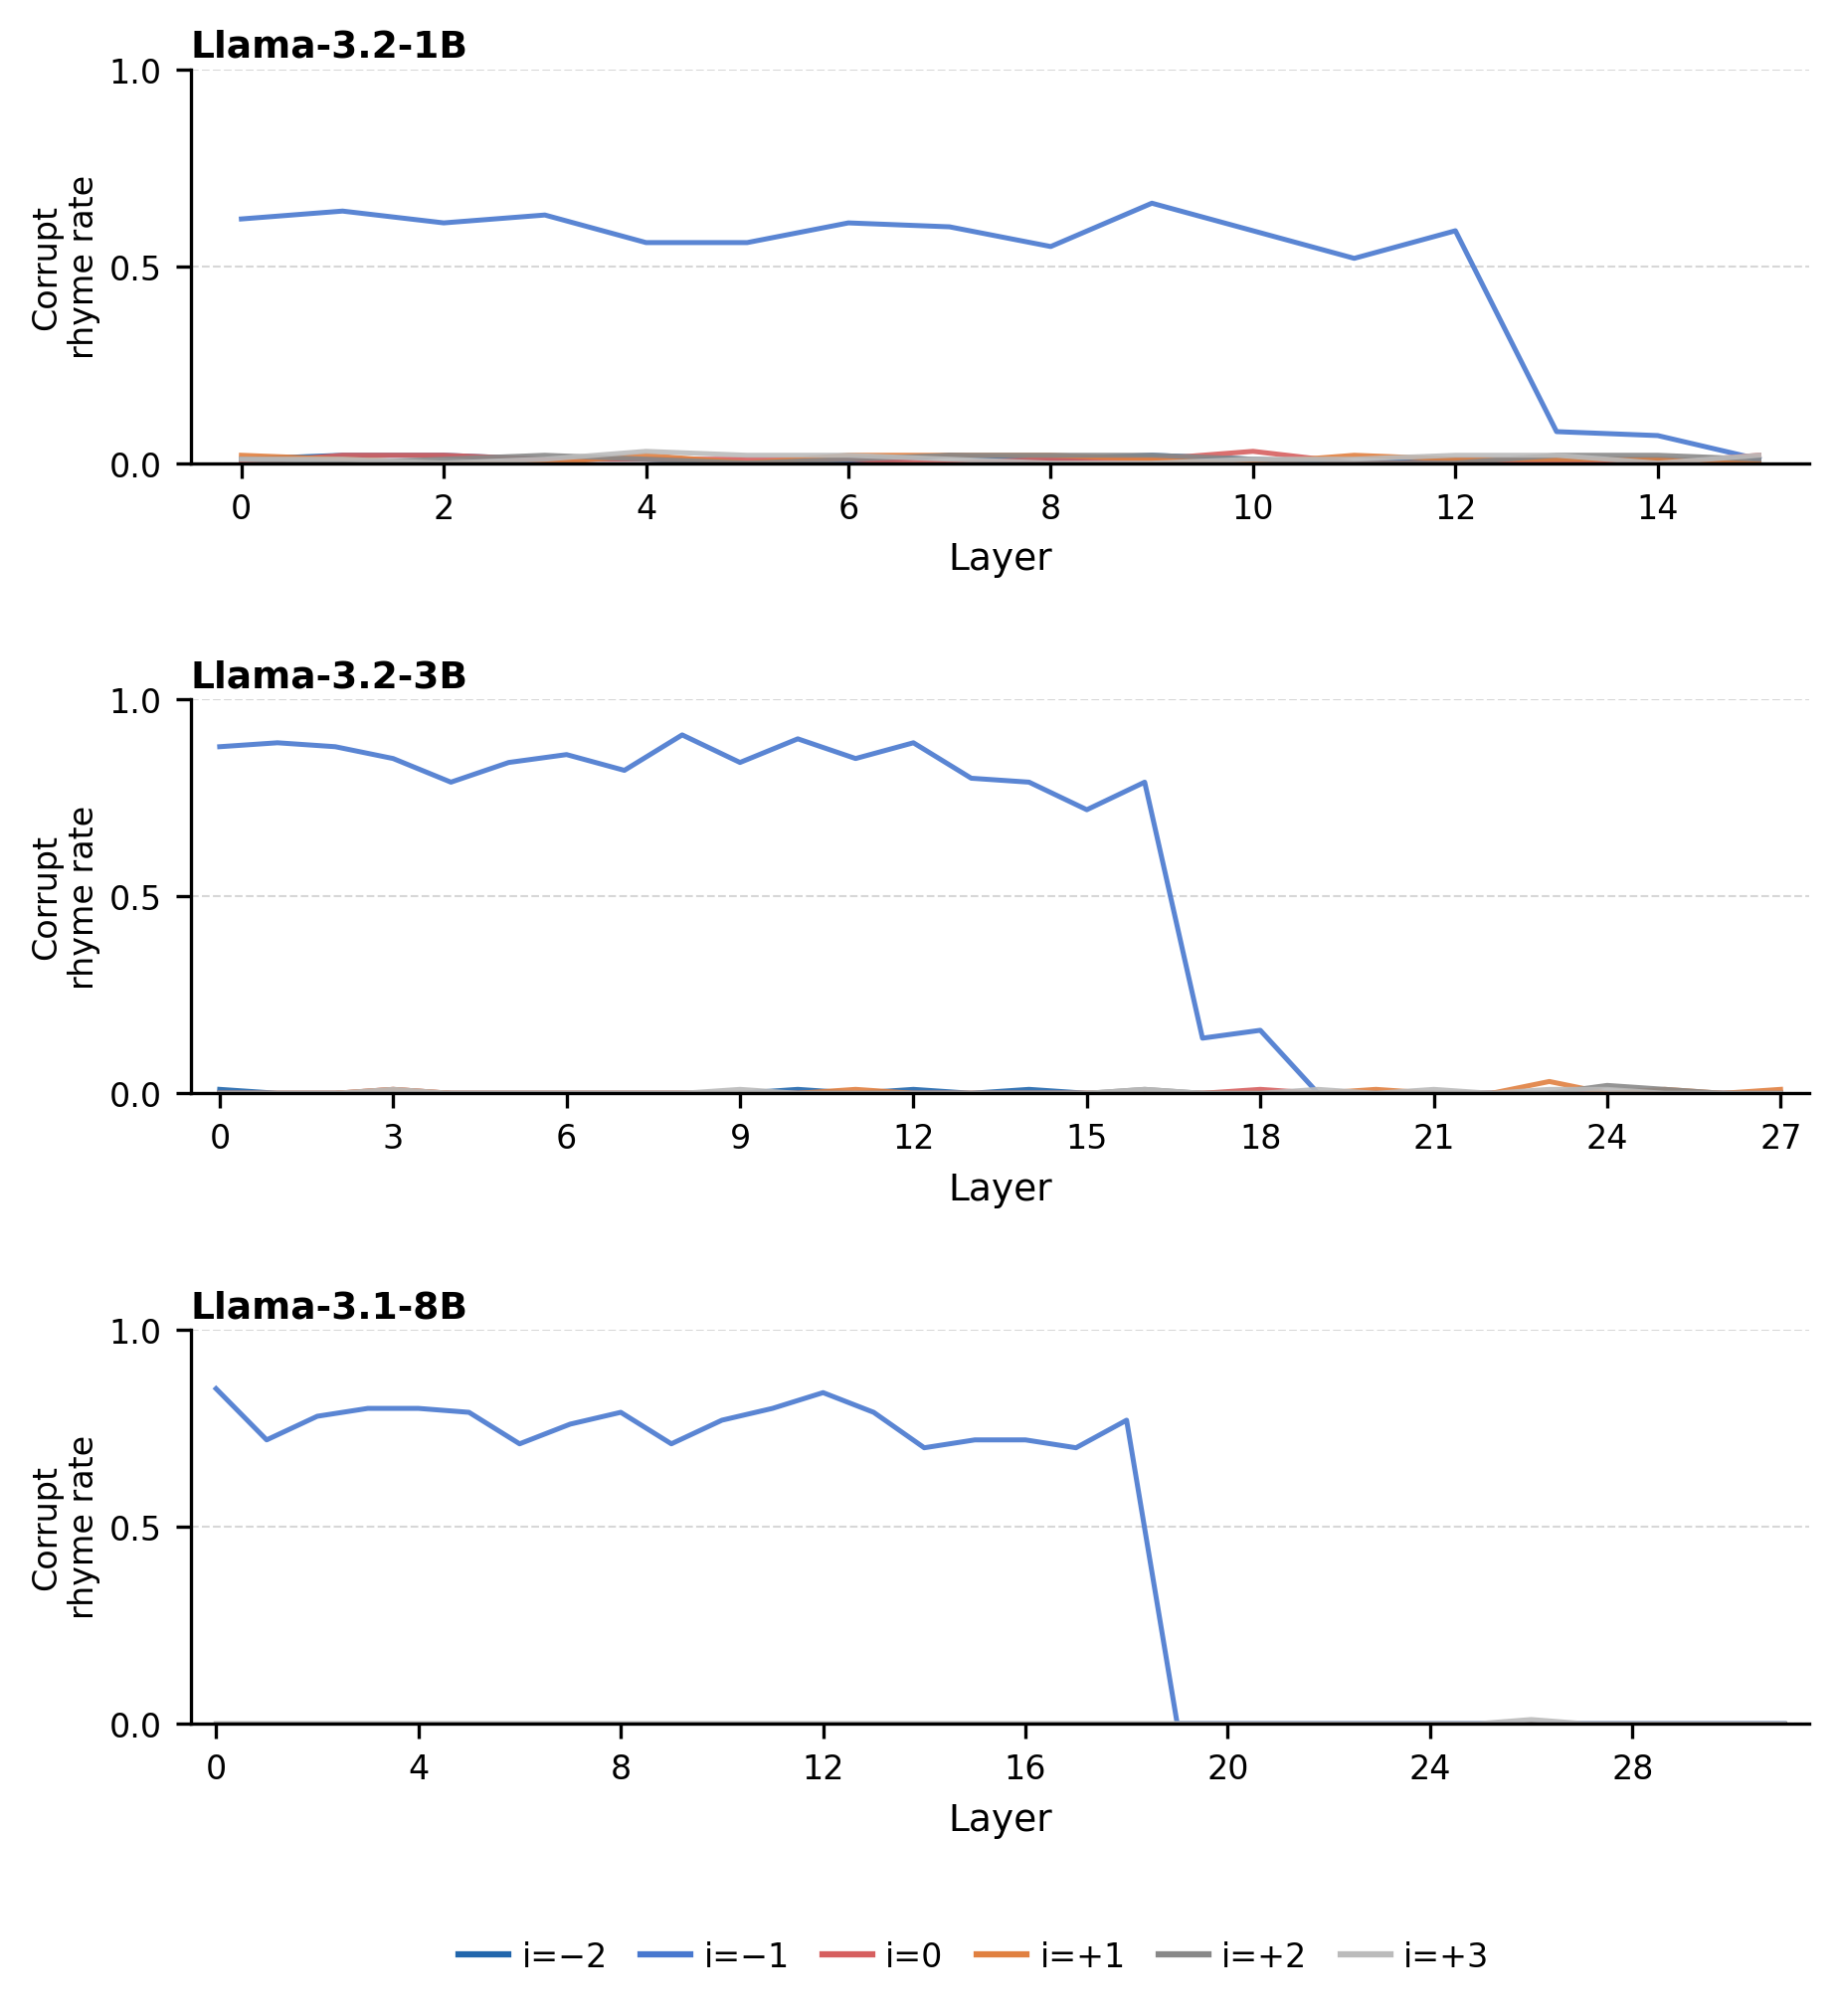
\includegraphics[width=\linewidth]{media/results-patching/appendix_sweep_Llama3.png}
    \caption{Full position sweep, Llama-3 1B--8B.}
    \label{fig:appendix-sweep-llama3}
\end{figure}

\subsection*{Prompt Pairs}

For each pair, we show the clean prompt, the corrupt prompt, and an example patched completion
where activation patching was successful in steering the rhyme scheme.

{\small\raggedright
\medskip\noindent\textbf{Pair 1: doom/dread, $\ell=10$, $i=-1$}\\
\textit{Clean:} \texttt{...filled with silent doom,\textbackslash n when suddenly they}\\
\textit{Corrupt:} \texttt{...filled with silent dread,\textbackslash n when suddenly they}\\
\textit{Patched:} \texttt{when suddenly they heard a creaking bed.}

\medskip\noindent\textbf{Pair 2: bliss/joy, $\ell=1$, $i=-2$}\\
\textit{Clean:} \texttt{...The children laughed in bliss,\textbackslash n until they all}\\
\textit{Corrupt:} \texttt{...The children laughed in joy,\textbackslash n until they all}\\
\textit{Patched:} \texttt{until they all became a toy.}

\medskip\noindent\textbf{Pair 3: dark/night, $\ell=0$, $i=-2$}\\
\textit{Clean:} \texttt{...She wandered home alone into the dark,\textbackslash n and then she}\\
\textit{Corrupt:} \texttt{...She wandered home alone into the night,\textbackslash n and then she}\\
\textit{Patched:} \texttt{and then she saw a strange and eerie light.}

\medskip\noindent\textbf{Pair 4: grief/pain, $\ell=2$, $i=-1$}\\
\textit{Clean:} \texttt{...I never knew the depth of such grief,\textbackslash n as though the}\\
\textit{Corrupt:} \texttt{...I never knew the depth of such pain,\textbackslash n as though the}\\
\textit{Patched:} \texttt{as though the sky had lost its rain.}

\medskip\noindent\textbf{Pair 5: fright/fear, $\ell=1$, $i=-1$}\\
\textit{Clean:} \texttt{...She felt a sudden sense of fright,\textbackslash n and hoped that}\\
\textit{Corrupt:} \texttt{...She felt a sudden sense of fear,\textbackslash n and hoped that}\\
\textit{Patched:} \texttt{and hoped that someone would appear.}
}

\begin{figure}[H]
    \centering
    \begin{subfigure}{0.49\linewidth}
        \centering
        \subcaption[]{Qwen3-32B}
        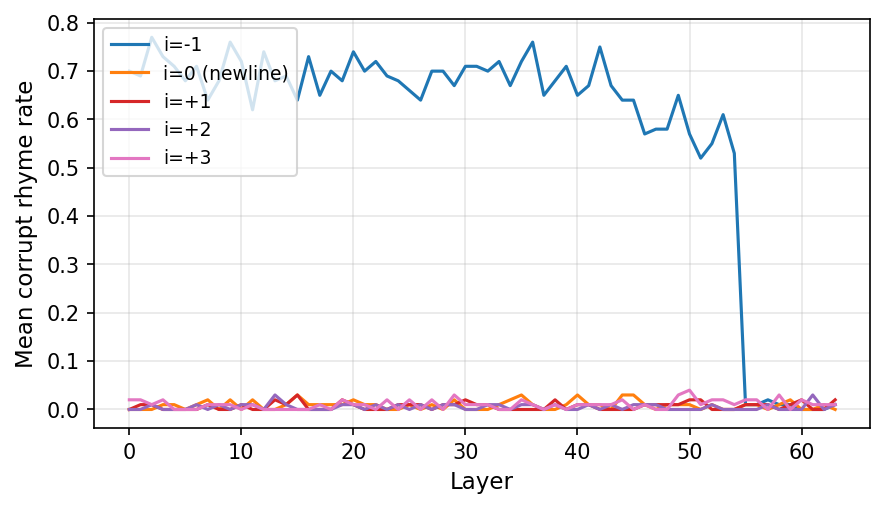
\includegraphics[width=\linewidth]{media/results-patching/qwen3_32b_aggregate_overlay.png}
    \end{subfigure}
    \begin{subfigure}{0.49\linewidth}
        \centering
        \subcaption[]{Gemma-3-27B}
        
\includegraphics[width=\linewidth]{media/results-patching/gemma3_27b_aggregate_overlay.png}
    \end{subfigure}
    \caption{Corrupt rhyme rate across all six swept token positions, averaged over 5 prompt pairs. For Gemma-3-27B, the comma token at $i=-1$ is near zero throughout, confirming the handoff is specific to the newline token.}
    \label{fig:patching-all-positions}
\end{figure}

\end{document}
